\chapter{Resultados}\label{chapter:resultados}

\section{Selección del framework de simulación SNN}
\label{sec:benchmark-framework-resultados}

En esta sección se presentan los resultados cuantitativos utilizados para comparar los frameworks \textit{ANNarchy}, \textit{NEST} y \textit{snn-simulator}, siguiendo el diseño experimental y el plan de análisis descritos en \ref{sec:benchmark-framework-metodologia}.

\paragraph{Tiempo de evaluación y comparación estadística}

La Figura~\ref{fig:eval-time-frameworks} muestra los resultados del tiempo de evaluación de la función objetivo para cada combinación de configuración y framework con 30 repeticiones en todas las configuraciones. Los resultados en detalle se encuentran en la Tabla \ref{tab:framework-evals-res}.

\begin{figure}
    \centering
    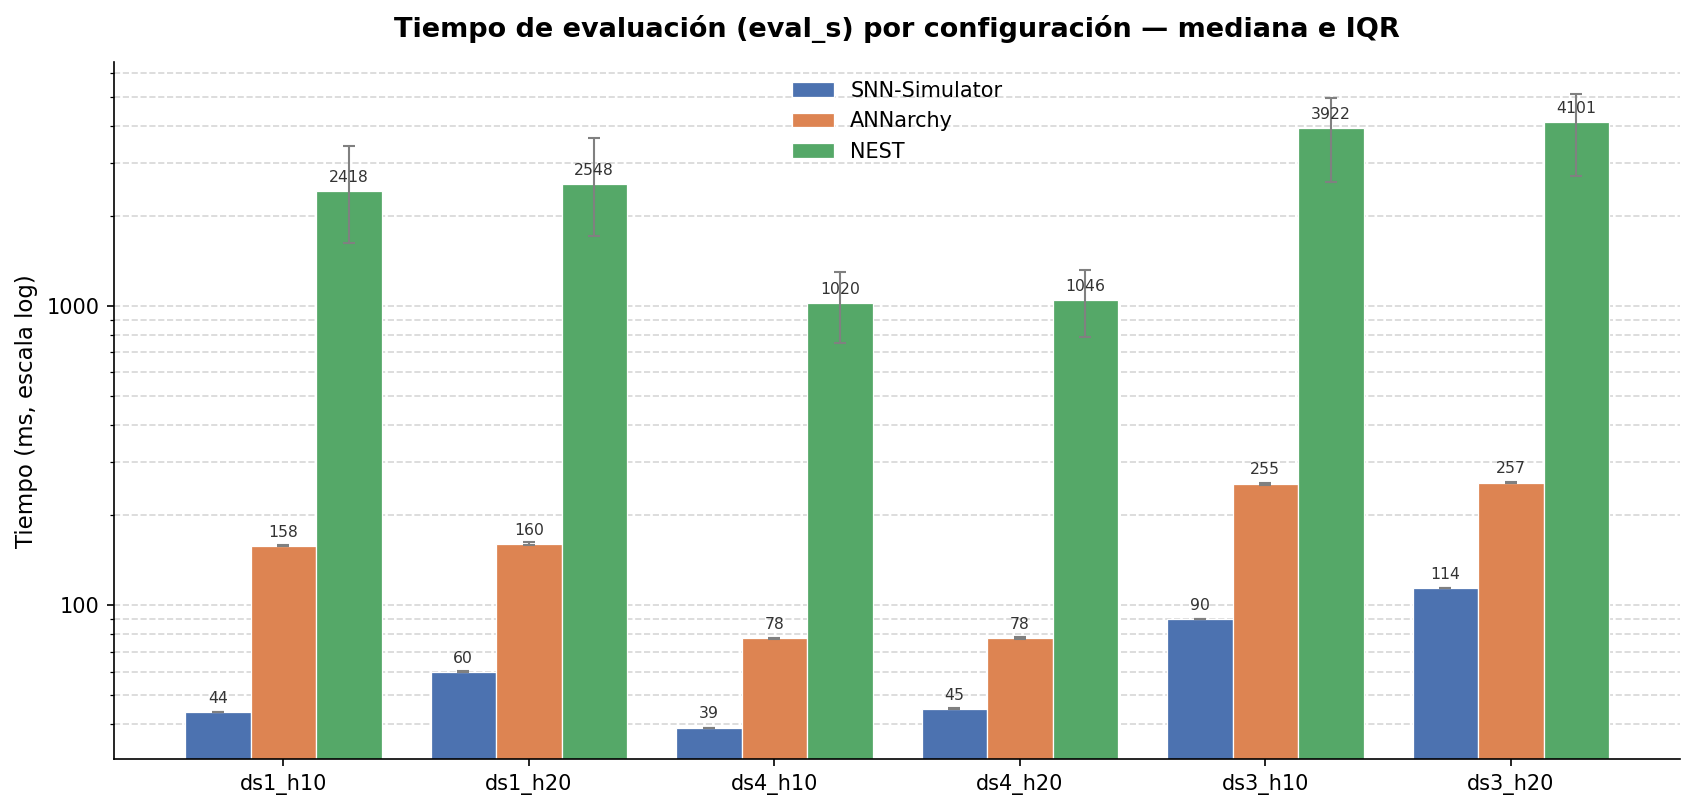
\includegraphics[width=0.8\linewidth]{images/plot_eval_s_median_iqr.png}
    \caption{Tiempo de evaluación por configuración y framework.}
    \label{fig:eval-time-frameworks}
\end{figure}

% En las seis configuraciones probadas se mantuvo el orden \textit{snn-simulator} \(<\) ANNarchy \(<\) NEST. Ordenando las seis configuraciones por dimensionalidad $D$, el ratio de velocidad \textit{snn-simulator} vs. cada competidor decrece de forma monótona: frente a ANNarchy, va de 3.58x (\texttt{ds1\_h10}, $D=160$) a 1.72x (\texttt{ds4\_h20}, $D=1240$); frente a NEST, de 54.9x ($D=160$) a 23.2x ($D=1240$). El patrón se sostuvo tanto al aumentar el número de neuronas en la capa oculta (de 10 a 20 neuronas dentro del mismo dataset) como al aumentar el número de características (mismo \texttt{nHidden}, distinto dataset), sin que este benchmark mostrara cuál de las dos dimensiones pesa más. Para el rango de $D$ efectivamente usado en esta prueba, \textit{snn-simulator} nunca deja de ser la opción más rápida por un margen amplio. Sin embargo, extrapolar la ventaja observada aquí a dimensiones muy superiores no está garantizado por estos datos.

% Ordenando las seis configuraciones por dimensionalidad $D$, el ratio de medianas de \textit{snn-simulator} frente a cada competidor decrece de forma monótona: frente a ANNarchy, va de 3.58x (\texttt{ds1\_h10}, $D=160$) a 1.72x (\texttt{ds4\_h20}, $D=1240$); frente a NEST, de 54.9x ($D=160$) a 23.2x ($D=1240$).

En las seis configuraciones probadas se mantuvo el mismo orden en tiempo de ejecución: \textit{snn-simulator} \(<\) ANNarchy \(<\) NEST. El patrón se sostuvo tanto al aumentar el número de neuronas en la capa oculta (de 10 a 20 neuronas dentro del mismo dataset) como al aumentar el número de características, sin que este benchmark mostrara cuál de las dos dimensiones pesa más. Se reporta la mediana debido al uso de la prueba no paramétrica de Mann-Whitney U. Para el rango de $D$ efectivamente usado en esta prueba, \textit{snn-simulator} nunca deja de ser la opción más rápida por un margen amplio. Sin embargo, extrapolar la ventaja observada aquí a dimensiones muy superiores no está garantizado por estos datos.


% \subsection{Comparación estadística entre frameworks (Mann-Whitney U)}

La Tabla~\ref{tab:framework-mannwhitney-res} resume las diferencias entre \textit{snn-simulator} y cada competidor, en base a la mediana, junto con el valor \(p\) de la prueba Mann-Whitney U, con 30 ejecuciones. Las 18 comparaciones por pares (tres frameworks por seis configuraciones) arrojan \(U = 0\) y separación total de las distribuciones, con \(p \approx 3{.}0 \times 10^{-11}\) en todos los casos. La comparación ANNarchy frente a NEST, no mostrada en la tabla, también resulta significativa a favor de ANNarchy en todas las configuraciones.

\begin{table}[htbp]
\centering
\small
\caption{Comparaciones por pares mediante Mann-Whitney \(U\). Las diferencias corresponden a la mediana de \textit{snn-simulator} menos la del competidor.}
\label{tab:framework-mannwhitney-res}
\begin{tabular}{lrrrr}
\toprule
Config & $\Delta$ vs ANNarchy (ms) & $p$ & $\Delta$ vs NEST (ms) & $p$ \\
\midrule
ds1\_h10 & -113.85 & $<0.0001$ & -2374.07 & $<0.0001$ \\
ds1\_h20 & -100.13 & $<0.0001$ & -2487.99 & $<0.0001$ \\
ds4\_h10 &  -38.47 & $<0.0001$ &  -980.50 & $<0.0001$ \\
ds4\_h20 &  -32.41 & $<0.0001$ & -1001.07 & $<0.0001$ \\
ds3\_h10 & -165.10 & $<0.0001$ & -3832.01 & $<0.0001$ \\
ds3\_h20 & -142.74 & $<0.0001$ & -3986.35 & $<0.0001$ \\
\bottomrule
\end{tabular}
\end{table}

El \textit{p-valor} indica que la diferencia no es producto del azar, pero no cuantifica qué tan grande es. De las 900 comparaciones posibles entre una medición de \textit{snn-simulator} y una del competidor ($30\times30$), \textit{snn-simulator} fue menor en las 900, sin un solo caso de solapamiento. No es un caso límite cercano a $p=0.05$, sino una diferencia que se sostiene en el 100\% de las 18 comparaciones. %(3 pares × 6 configs).

\paragraph{Tiempo de construcción y escalabilidad de la red}

La Figura \ref{fig:build_s_by_config} muestra el tiempo de construcción de la red por cada framework en las seis configuraciones con 30 repeticiones en cada una. El \textit{snn-simulator} construye la red en microsegundos, entre tres y cuatro órdenes de magnitud más rápido que NEST y ANNarchy. ANNarchy incurre además en un costo adicional de compilación Cython de aproximadamente 9{.}6–9{.}8 segundos por corrida. Los resultados completos se pueden visualizar en la Tabla \ref{tab:framework-build-memory-res} del Anexo.

\begin{figure}
    \centering
    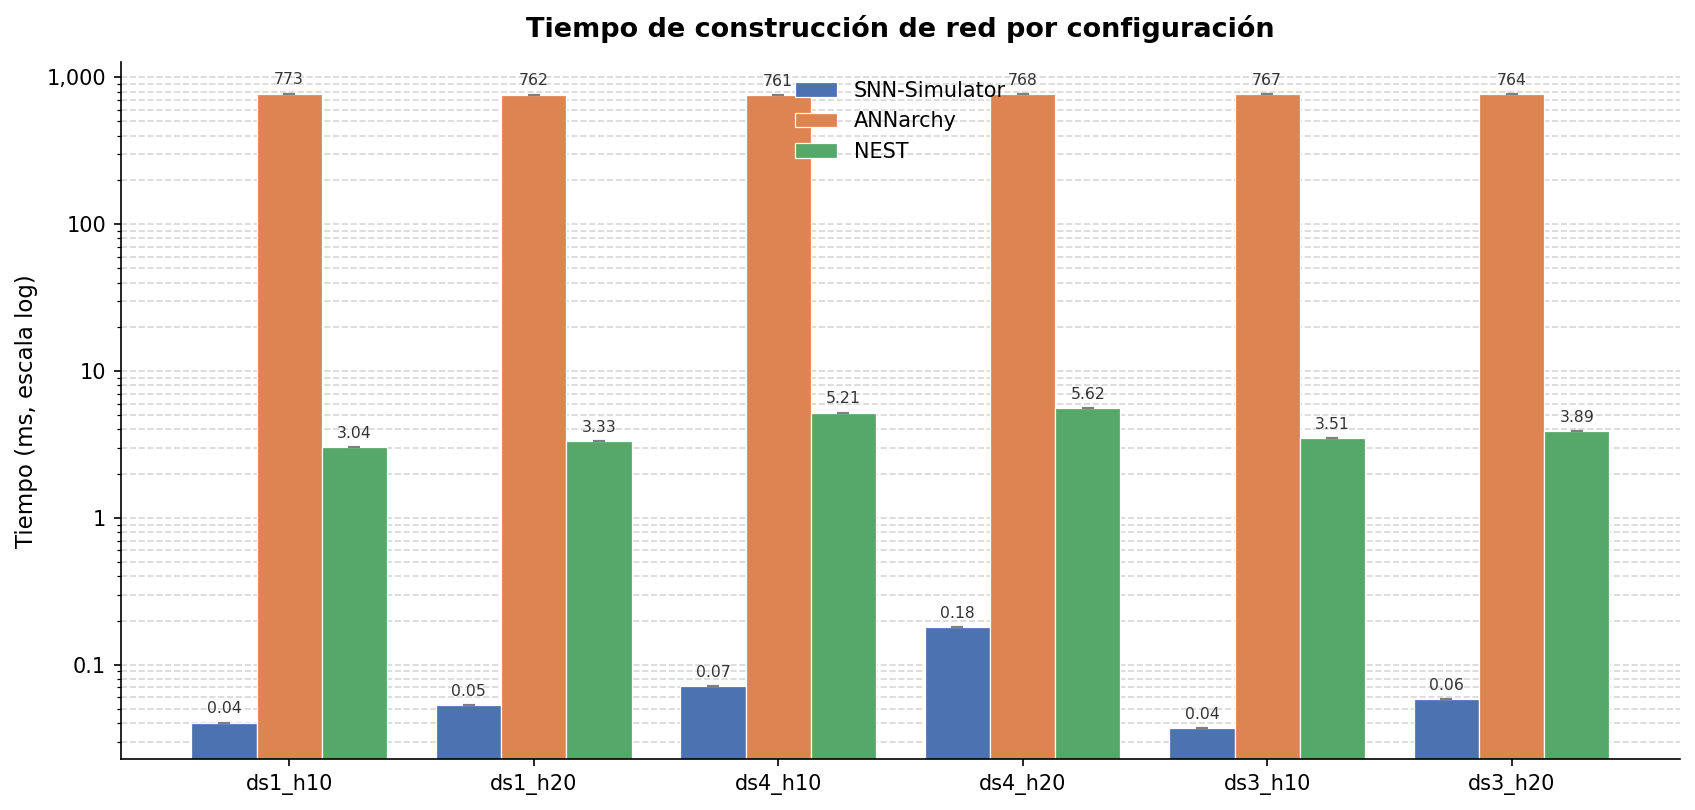
\includegraphics[width=0.8\linewidth]{images/plot_build_s_by_config.png}
    \caption{Tiempo de construcción por configuración y framework.}
    \label{fig:build_s_by_config}
\end{figure}

% \subsection{Overhead puro del algoritmo evolutivo}

% La Tabla~\ref{tab:framework-moea-overhead-res} resume el tiempo de ejecución de MOEA-CKF y S-NSGA-II sin simulador real (problema trivial), junto con la razón entre ambos.

% \begin{table}[htbp]
% \centering
% \small
% \caption{Overhead de los algoritmos evolutivos sin simulador.}
% \label{tab:framework-moea-overhead-res}
% \begin{tabular}{lrrrr}
% \toprule
% Config & $D$ & MOEACKF (s) & SNSGAII (s) & Razón MOEACKF/SNSGAII \\
% \midrule
% ds1\_h10 & 160  &  4.18 & 0.082 &  51.1$\times$ \\
% ds1\_h20 & 320  & 17.57 & 0.143 & 123.2$\times$ \\
% ds4\_h10 & 620  & 82.26 & 0.255 & 322.3$\times$ \\
% ds4\_h20 & 1240 & 222.19 & 0.503 & 442.1$\times$ \\
% ds3\_h10 & 260  & 12.39 & 0.121 & 102.4$\times$ \\
% ds3\_h20 & 520  & 61.25 & 0.215 & 284.4$\times$ \\
% \bottomrule
% \end{tabular}
% \end{table}

% MOEA-CKF escala mucho peor con la dimensionalidad \(D\) del vector de pesos que S-NSGA-II, y este overhead se suma al costo de simulación independientemente del framework elegido.

\paragraph{Selección del framework}

Con base en los resultados anteriores, se selecciona \textit{snn-simulator} como framework de simulación SNN para el pipeline de entrenamiento. La decisión se apoya en: (i) tiempos de evaluación significativamente menores en las seis configuraciones, con separación completa de las distribuciones frente a ANNarchy y NEST, y (ii) tiempos de construcción varios órdenes de magnitud inferiores sin compilación adicional.

La principal desventaja de \textit{snn-simulator} es un consumo de memoria aproximadamente 9 MB superior al de ANNarchy en las configuraciones evaluadas, siendo esta diferencia irrelevante frente a la ventaja temporal de dos a tres órdenes de magnitud y frente al hecho de que la memoria de \textit{snn-simulator} se mantiene estable mientras que la de NEST crece con el número de evaluaciones.

Las amenazas a la validez incluyen la anomalía confirmada de tendencia en NEST (crecimiento monótono del tiempo de evaluación al duplicar el número de repeticiones dentro del mismo proceso), y la realización de mediciones en una sola máquina y sesión diferente a donde se realizaron los experimentos finales.


%---------------

\section{Resultados de la búsqueda de hiperparámetros}

Siguiendo la metodología descrita en la Sección~\ref{sec:metodologia_busqueda_hiper}, se ejecutaron ocho estudios independientes de búsqueda de hiperparámetros, uno por cada algoritmo sobre los datasets seleccionados.

La Tabla \ref{tab:hv_por_dataset_resultados} resume el HV medio de la mejor configuración encontrada en cada estudio, junto con el \emph{trial} ganador y la arquitectura asociada. En todos los casos, la configuración ganadora corresponde a redes con dos neuronas de salida con codificación Poisson o TTFS según el dataset y el algoritmo.

% Please add the following required packages to your document preamble:
% \usepackage{multirow}
\begin{table}[htbp]
\centering
\small
\caption{Mejor HV medio, promediado sobre configuraciones de 20, 40 y 80 neuronas, por algoritmo y conjunto de datos. La arquitectura es la seleccionada mediante la búsqueda de hiperparámetros.}
\label{tab:hv_por_dataset_resultados}
\begin{tabular}{ccclccl}
\hline
\textbf{Dataset}            & \textbf{Características}     & \textbf{maxFE}                    & \textbf{Algoritmo} & \textbf{HV medio} & \textbf{Trial}& \textbf{Arquitectura} \\ \hline
\multirow{2}{*}{1} & \multirow{2}{*}{14} & \multirow{2}{*}{9\,900}  & MOEA-CKF  & 0.8707   & 50    & Poisson             \\
                   &                     &                          & S-NSGA-II & 0.8742   & 17    & TTFS                \\ \hline
\multirow{2}{*}{2} & \multirow{2}{*}{18} & \multirow{2}{*}{11\,500} & MOEA-CKF  & 0.9297   & 31    & TTFS                \\
                   &                     &                          & S-NSGA-II & 0.9291   & 44    & Poisson             \\ \hline
\multirow{2}{*}{3} & \multirow{2}{*}{24} & \multirow{2}{*}{13\,900} & MOEA-CKF  & 0.7501   & 40    & TTFS                \\
                   &                     &                          & S-NSGA-II & 0.7550   & 24    & Poisson             \\ \hline
\multirow{2}{*}{4} & \multirow{2}{*}{60} & \multirow{2}{*}{28\,300} & MOEA-CKF  & 0.8008   & 59    & TTFS                \\
                   &                     &                          & S-NSGA-II & 0.8268   & 11    & TTFS   \\ \hline
\end{tabular}
\end{table}

\subsection{Resultados por dataset}

\subsubsection{Dataset 1: Statlog Australian}

Ambos algoritmos alcanzan un HV medio muy similar en sus mejores configuraciones: 0.8707 para MOEA-CKF y 0.8742 para S-NSGA-II. La diferencia principal es el codificador, Poisson en MOEA-CKF y TTFS en S-NSGA-II. Estas configuraciones se detallan en la Tabla~\ref{tab:hiper_mejor_config}, donde se observa además que los índices de distribución de cruce y mutación, así como los parámetros de esparsidad, adoptan valores distintos entre algoritmos.

\begin{table}[htbp]
    \centering
    \small
    \caption{Hiperparámetros de la mejor configuración por algoritmo y dataset.}
    \label{tab:hiper_mejor_config}
    \resizebox{\textwidth}{!}{%
        \begin{tabular}{lcccccccc}
            \hline
            Parámetro &
            ds1-CKF &
            ds1-NSGA &
            ds2-CKF &
            ds2-NSGA &
            ds3-CKF &
            ds3-NSGA &
            ds4-CKF &
            ds4-NSGA \\
            \hline
            disC   & 28.01 & 16.61 & 9.90  & 5.03  & 99.85 & 9.84  & 74.56 & 6.01  \\
            disM   & 28.35 & 9.55  & 8.04  & 50.62 & 21.35 & 8.14  & 5.66  & 56.64 \\
            proM   & 1.79  & 2.99  & 2.07  & 2.90  & 0.74  & 2.44  & 0.58  & 1.66  \\
            disSM  & 25.44 & 35.44 & 18.60 & 61.71 & 6.00  & 63.25 & 6.49  & 82.44 \\
            proSM  & 1.02  & 1.69  & 2.34  & 1.49  & 1.21  & 0.99  & 1.47  & 2.67  \\
            sLower & 0.81  & 0.66  & 0.54  & 0.85  & 0.88  & 0.69  & 0.70  & 0.63  \\
            sGap   & 0.12  & 0.23  & 0.26  & 0.30  & 0.25  & 0.27  & 0.07  & 0.05  \\
            wScale & 34.75 & 13.63 & 8.99  & 44.41 & 36.96 & 16.42 & 27.12 & 40.27 \\
            \hline
        \end{tabular}%
    }
\end{table}

Las trayectorias de convergencia del HV medio por \emph{trial} muestran que ambos estudios sobre el dataset 1 convergen de manera estable hacia el final de los 60 trials, donde se aprecia que MOEA-CKF y S-NSGA-II aprovechan de forma similar el presupuesto de \texttt{maxFE} compartido. Este comportamiento se ilustra en las Figuras~\ref{fig:ds1_convergencia_ckf} y~\ref{fig:ds1_convergencia_nsga}.

\begin{figure}[htbp]
    \centering

    \begin{subfigure}[b]{0.48\textwidth}
        \centering
        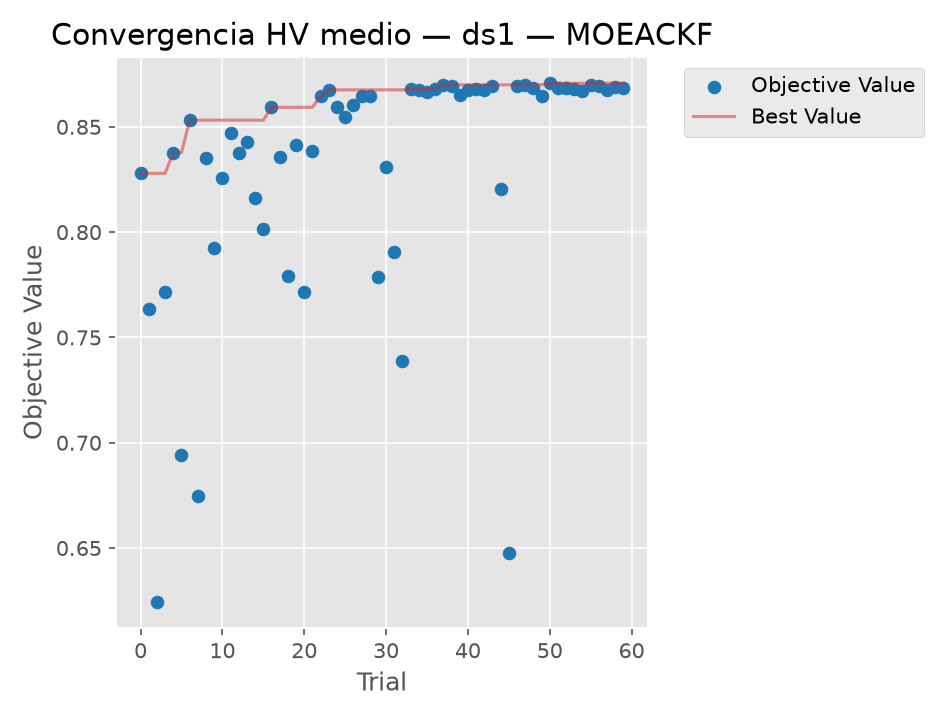
\includegraphics[width=\textwidth]{images/convergencia_MOEACKF_ds1.png}
        \caption{HV medio por trial en \texttt{ds1} para MOEA-CKF.}
        \label{fig:ds1_convergencia_ckf}
    \end{subfigure}
    \hfill
    \begin{subfigure}[b]{0.48\textwidth}
        \centering
        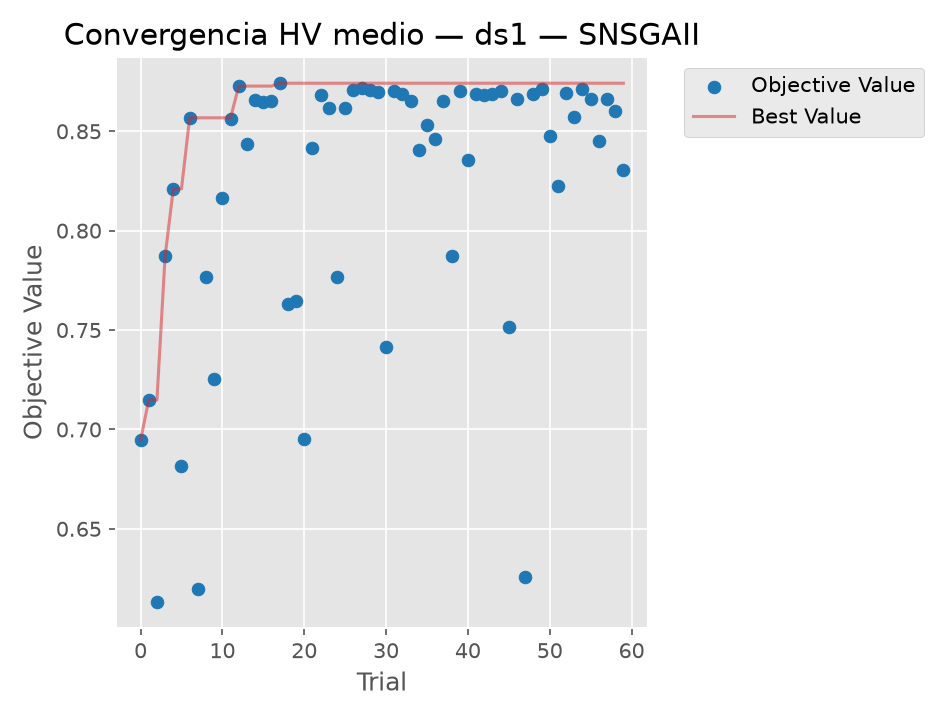
\includegraphics[width=\textwidth]{images/convergencia_SNSGAII_ds1.png}
        \caption{HV medio por \emph{trial} en \texttt{ds1} para S-NSGA-II.}
        \label{fig:ds1_convergencia_nsga}
    \end{subfigure}

    \caption{Convergencia del hipervolumen entre ambos algoritmos para el dataset 1.}
    \label{fig:comparacion_hv_ds1}
\end{figure}

El análisis de importancia de hiperparámetros en \texttt{ds1} muestra que \texttt{wScale} concentra la mayor parte de la varianza explicada del HV en ambos algoritmos, de forma casi absoluta en MOEA-CKF (94.7\%) y más repartida en S-NSGA-II (53.7\%), donde \texttt{sLower} aporta una contribución secundaria relevante (31.8\%). Estas relaciones se muestran en las Figuras~\ref{fig:ds1_fanova_ckf} y~\ref{fig:ds1_fanova_nsga}.

\begin{figure}[htbp]
    \centering
    \begin{subfigure}[b]{0.48\textwidth}
        \centering
        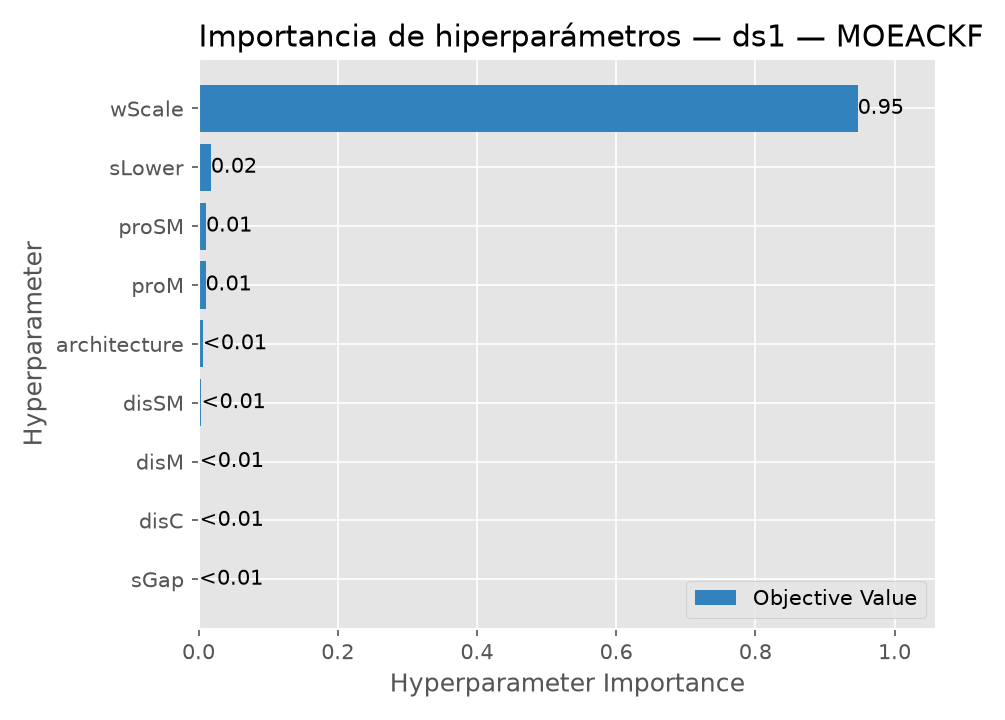
\includegraphics[width=\textwidth]{images/importancia_MOEACKF_ds1.png}
        \caption{Importancia de hiperparámetros (fANOVA) en \texttt{ds1} para MOEA-CKF (corresponde a la Figura~11).}
        \label{fig:ds1_fanova_ckf}
    \end{subfigure}
    \hfill
    \begin{subfigure}[b]{0.48\textwidth}
        \centering
        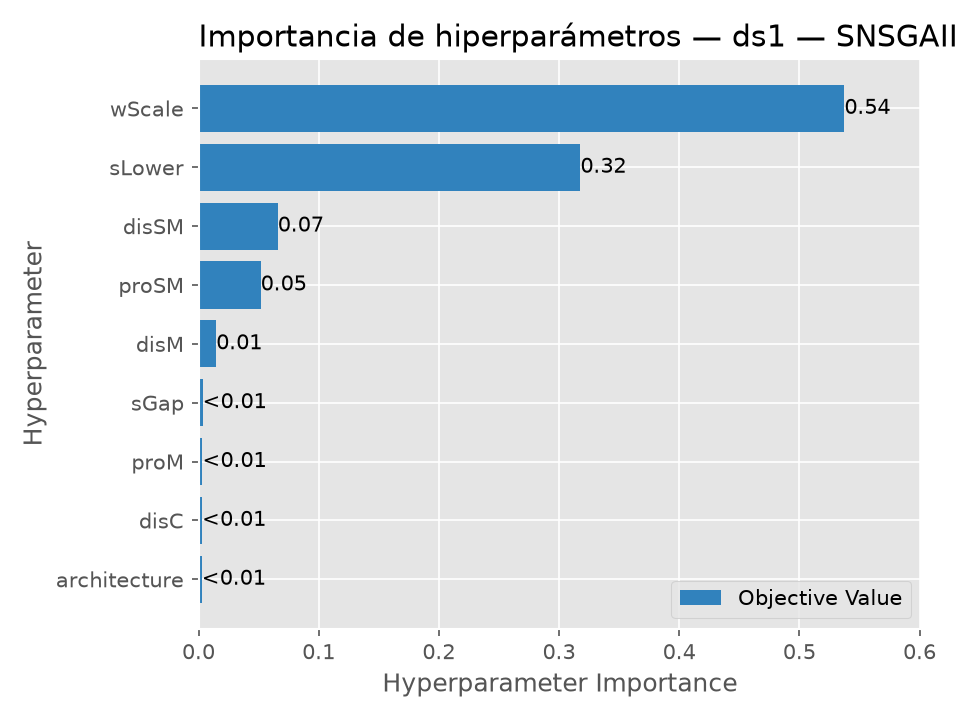
\includegraphics[width=\textwidth]{images/importancia_SNSGAII_ds1.png}
        \caption{Importancia de hiperparámetros (fANOVA) en \texttt{ds1} para S-NSGA-II (corresponde a la Figura~12).}
        \label{fig:ds1_fanova_nsga}
    \end{subfigure}

    \caption{Importancia de hiperparámetros en \texttt{ds1} para ambos algoritmos.}
    \label{fig:importancia_hiper_ds1}
\end{figure}

\subsubsection{Dataset 2: Climate}


Los mejores HV medios alcanzados en \texttt{ds2} son 0.9297 para MOEA-CKF y 0.9291 para S-NSGA-II. La configuración ganadora correspondió a TTFS en MOEA-CKF y Poisson en S-NSGA-II. Las Figuras~\ref{fig:ds2_convergencia_ckf} y~\ref{fig:ds2_convergencia_nsga} muestran la convergencia del HV medio por \emph{trial} para MOEA-CKF y S-NSGA-II en \texttt{ds2}, respectivamente, concentrando los HV en una banda alta y estrecha entre 0.91 y 0.93.

\begin{figure}[htbp]
    \centering
    \begin{subfigure}[b]{0.48\textwidth}
        \centering
        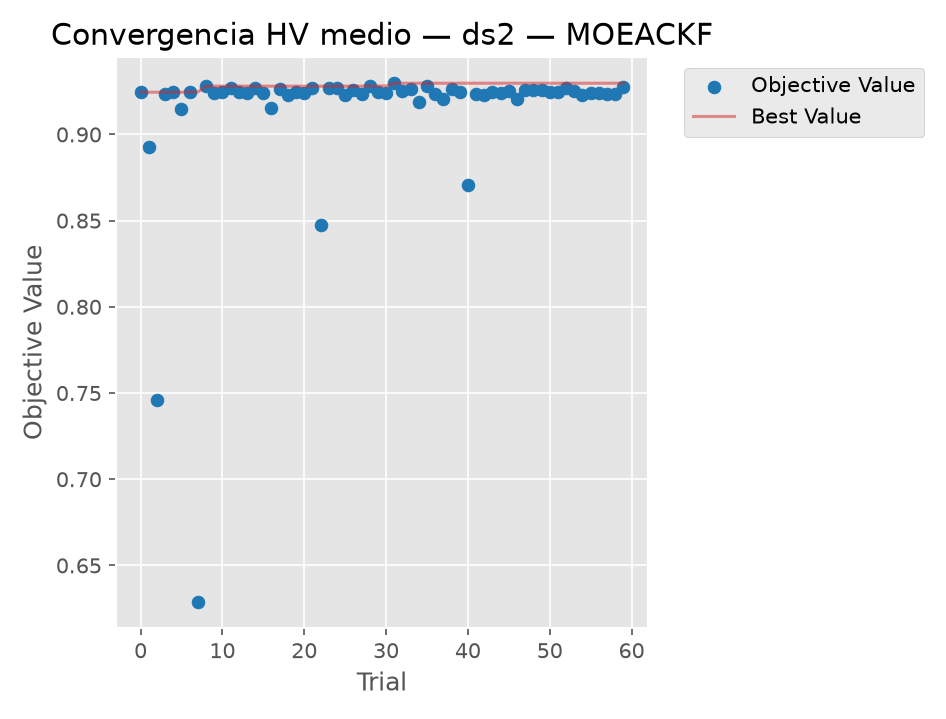
\includegraphics[width=\textwidth]{images/convergencia_MOEACKF_ds2.png}
        \caption{Convergencia del HV medio por \emph{trial} en \texttt{ds2} para MOEA-CKF.}
        \label{fig:ds2_convergencia_ckf}
    \end{subfigure}
    \hfill
    \begin{subfigure}[b]{0.48\textwidth}
        \centering
        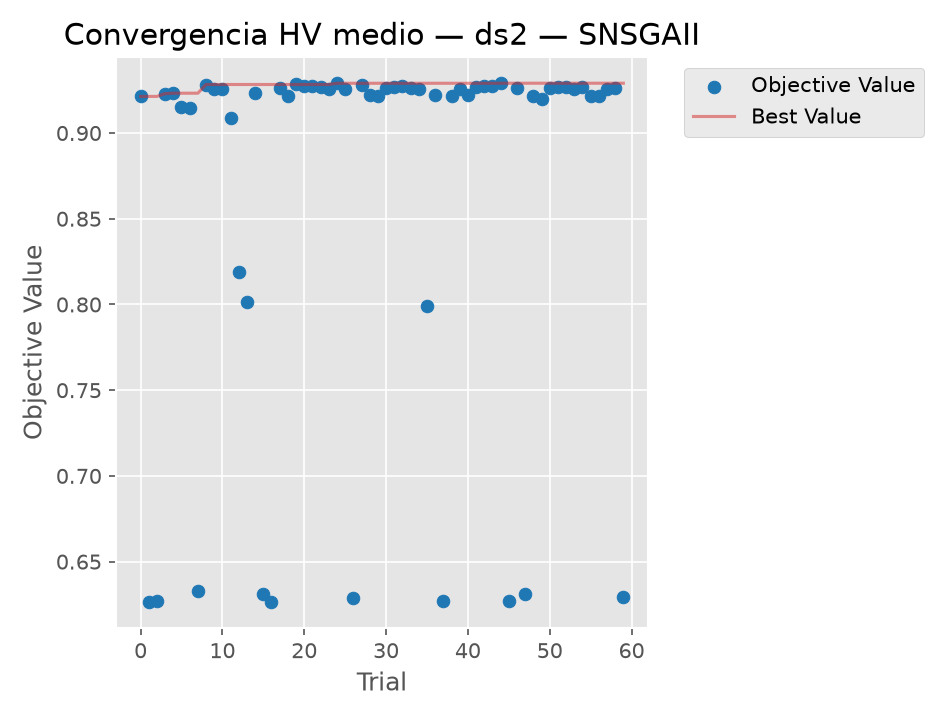
\includegraphics[width=\textwidth]{images/convergencia_SNSGAII_ds2.png}
        \caption{Convergencia del HV medio por \emph{trial} en \texttt{ds2} para S-NSGA-II.}
        \label{fig:ds2_convergencia_nsga}
    \end{subfigure}

    \caption{Comparación de convergencia del hipervolumen entre ambos algoritmos para el Dataset 2.}
    \label{fig:comparacion_hv_ds2}
\end{figure}

El análisis fANOVA en \texttt{ds2} muestra que, al igual que en \texttt{ds1}, es \texttt{wScale} quien concentra casi toda la varianza explicada del HV en ambos algoritmos (95.9\% en MOEA-CKF, 96.2\% en S-NSGA-II), mientras que \texttt{architecture} queda con una importancia prácticamente nula (por debajo del 0.2\% en ambos algoritmos), consistente con que ninguna de las dos resulte claramente superior a la otra en este dataset (Tabla~\ref{tab:hv_por_dataset_resultados}). Esta relación se ilustra en las Figuras~\ref{fig:ds2_fanova_ckf} y~\ref{fig:ds2_fanova_nsga}.

\begin{figure}[htbp]
    \centering

    \begin{subfigure}[b]{0.48\textwidth}
        \centering
        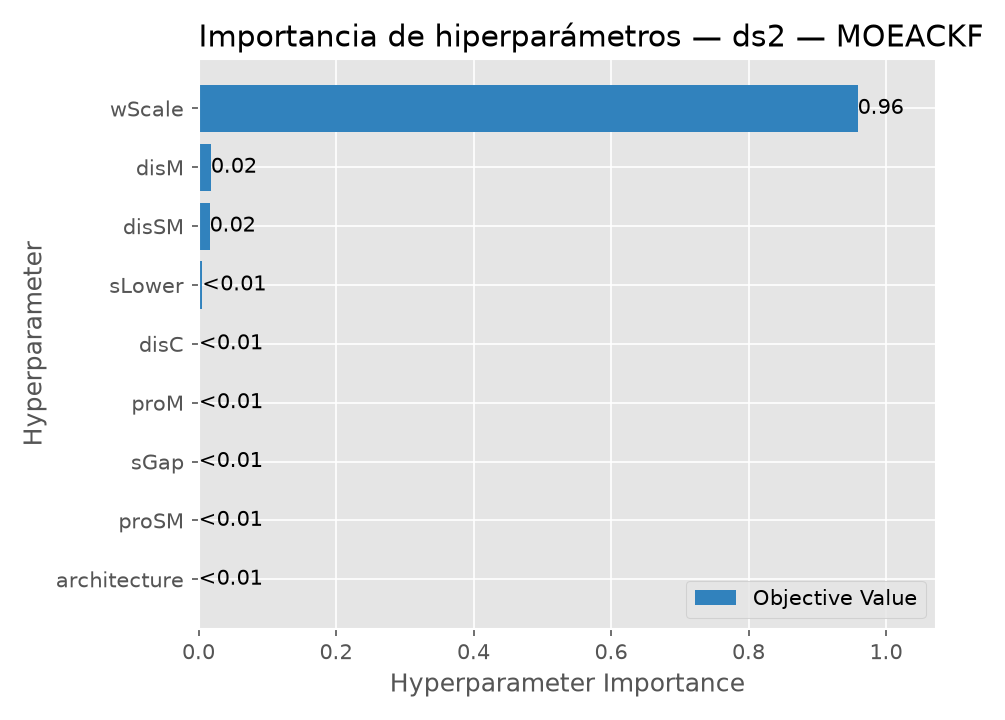
\includegraphics[width=\textwidth]{images/importancia_MOEACKF_ds2.png}
        \caption{Importancia de hiperparámetros (fANOVA) en \texttt{ds2} para MOEA-CKF.}
        \label{fig:ds2_fanova_ckf}
    \end{subfigure}
    \hfill
    \begin{subfigure}[b]{0.48\textwidth}
        \centering
        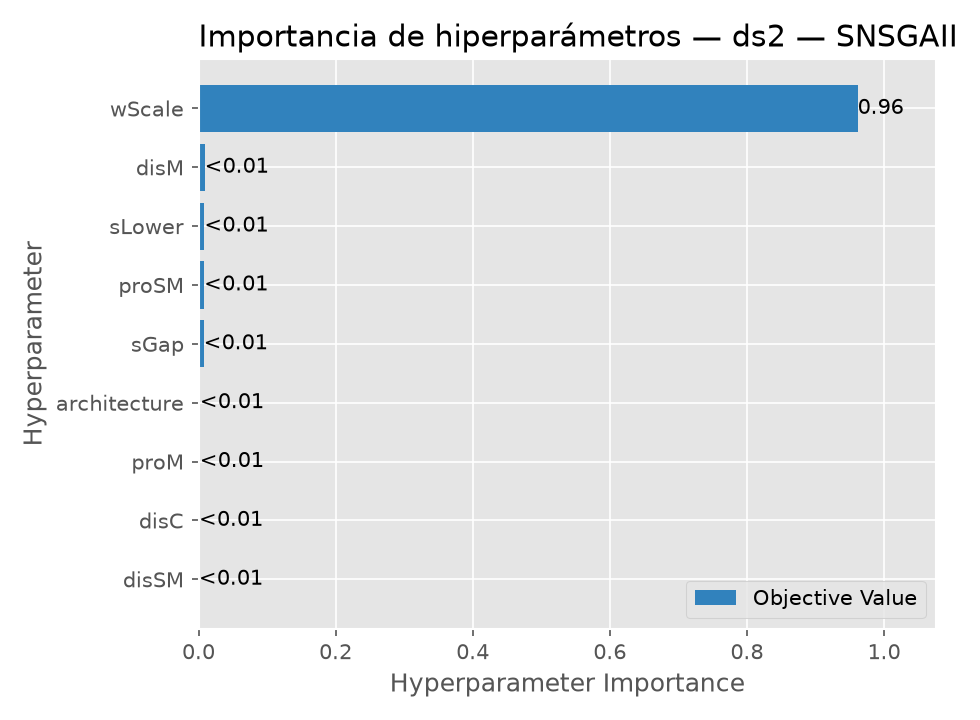
\includegraphics[width=\textwidth]{images/importancia_SNSGAII_ds2.png}
        \caption{Importancia de hiperparámetros (fANOVA) en \texttt{ds2} para S-NSGA-II.}
        \label{fig:ds2_fanova_nsga}
    \end{subfigure}

    \caption{Importancia de hiperparámetros en \texttt{ds2} para ambos algoritmos.}
    \label{fig:importancia_hiper_ds2}
\end{figure}

\subsubsection{Dataset 3: Statlog German}

En este dataset ambos algoritmos alcanzan un HV medio muy cercano, con S-NSGA-II por sobre MOEA-CKF (0.7550 frente a 0.7501). La Tabla~\ref{tab:hiper_mejor_config} muestra que ambas configuraciones difieren en varios hiperparámetros continuos, incluyendo \texttt{wScale} y los límites de esparsidad: MOEA-CKF selecciona una banda de esparsidad orientada a redes muy esparsas (\texttt{sLower} cercana a 0.88), mientras que S-NSGA-II opta por una banda algo más densa (\texttt{sLower}$\approx$0.69).

Las Figuras~\ref{fig:ds3_convergencia_ckf} y~\ref{fig:ds3_convergencia_nsga} ilustran las trayectorias de convergencia del HV medio por \emph{trial} en \texttt{ds3} para ambos algoritmos. Ambos estudios convergen de forma estable hacia el final de los 60 trials, con S-NSGA-II mostrando algo menos de dispersión entre trials cercanos al final de la búsqueda.

\begin{figure}[htbp]
    \centering
    \begin{subfigure}[b]{0.48\textwidth}
        \centering
        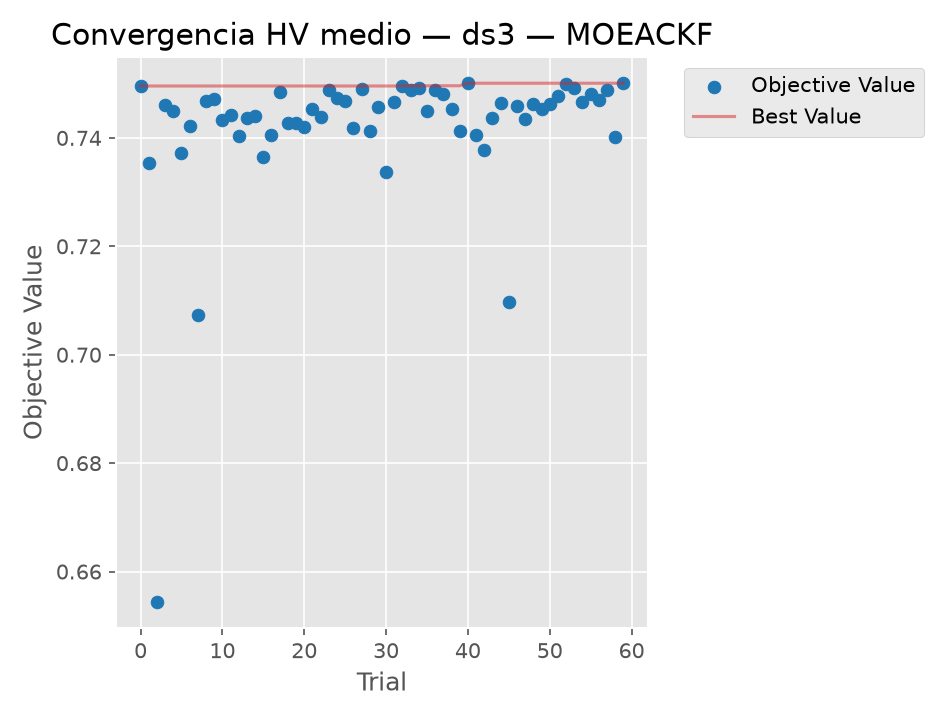
\includegraphics[width=\textwidth]{images/convergencia_MOEACKF_ds3.png}
        \caption{Convergencia del HV medio por \emph{trial} en \texttt{ds3} para MOEA-CKF.}
        \label{fig:ds3_convergencia_ckf}
    \end{subfigure}
    \hfill
    \begin{subfigure}[b]{0.48\textwidth}
        \centering
        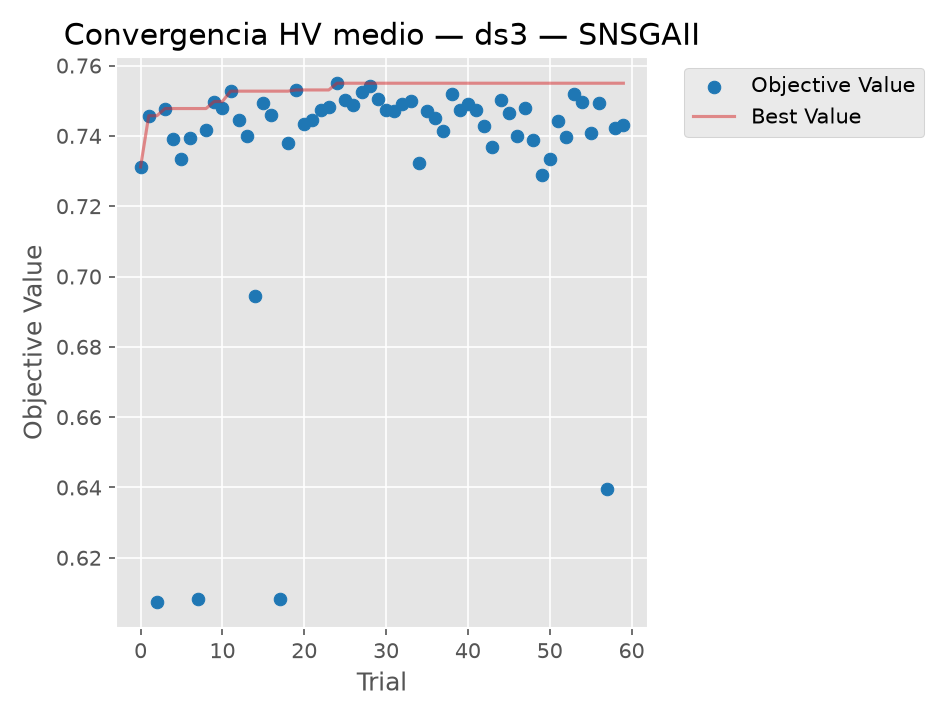
\includegraphics[width=\textwidth]{images/convergencia_SNSGAII_ds3.png}
        \caption{Convergencia del HV medio por \emph{trial} en \texttt{ds3} para S-NSGA-II.}
        \label{fig:ds3_convergencia_nsga}
    \end{subfigure}

    \caption{Comparación de convergencia del hipervolumen entre ambos algoritmos para el Dataset 3.}
    \label{fig:comparacion_hv_ds3}
\end{figure}

En cuanto a la importancia de hiperparámetros, el análisis fANOVA en \texttt{ds3} muestra que \texttt{wScale} vuelve a ser el hiperparámetro más influyente para ambos algoritmos (82.4\% en MOEA-CKF, 89.8\% en S-NSGA-II), con \texttt{proSM} como contribución secundaria en MOEA-CKF (11.4\%). Las Figuras~\ref{fig:ds3_fanova_ckf} y~\ref{fig:ds3_fanova_nsga} reflejan este patrón.

\begin{figure}[htbp]
    \centering

    \begin{subfigure}[b]{0.48\textwidth}
        \centering
        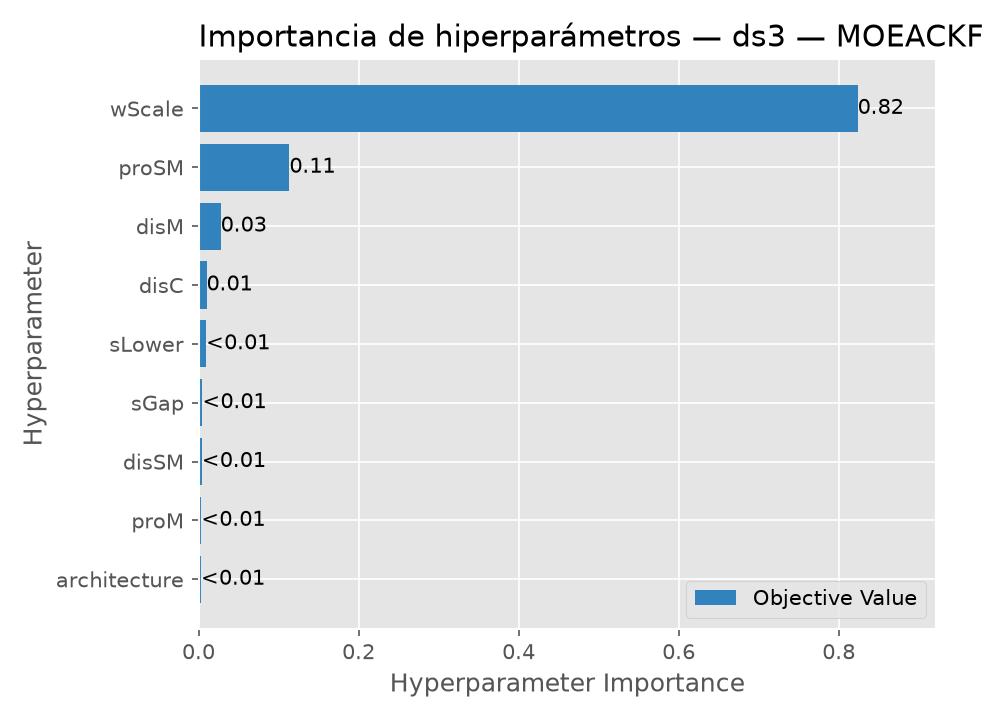
\includegraphics[width=\textwidth]{images/importancia_MOEACKF_ds3.png}
        \caption{Importancia de hiperparámetros (fANOVA) en \texttt{ds3} para MOEA-CKF.}
        \label{fig:ds3_fanova_ckf}
    \end{subfigure}
    \hfill
    \begin{subfigure}[b]{0.48\textwidth}
        \centering
        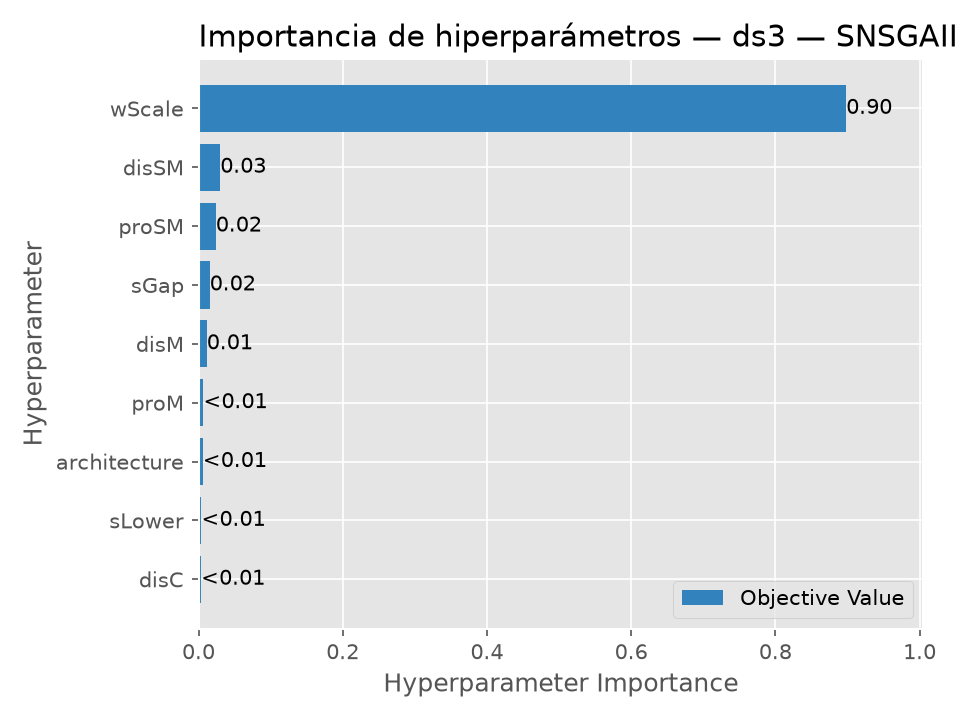
\includegraphics[width=\textwidth]{images/importancia_SNSGAII_ds3.png}
        \caption{Importancia de hiperparámetros (fANOVA) en \texttt{ds3} para S-NSGA-II.}
        \label{fig:ds3_fanova_nsga}
    \end{subfigure}

    \caption{Importancia de hiperparámetros en \texttt{ds3} para ambos algoritmos.}
    \label{fig:importancia_hiper_ds3}
\end{figure}

\subsubsection{Dataset 4: Connectionist Bench Sonar}

En este dataset S-NSGA-II supera a MOEA-CKF por el margen más amplio de los cuatro estudios, con HV medio 0.8268 frente a 0.8008. Las arquitecturas ganadoras tienen codificación TTFS en ambos casos, pero difieren en varios hiperparámetros continuos, incluyendo \texttt{wScale} y los parámetros de esparsidad.

Las Figuras~\ref{fig:ds4_convergencia_ckf} y~\ref{fig:ds4_convergencia_nsga} muestran las curvas de HV medio por \emph{trial} en \texttt{ds4}, evidenciando que tanto MOEA-CKF como S-NSGA-II logran convergencias estables y valores de HV comparables en las últimas iteraciones.

\begin{figure}[htbp]
    \centering
    \begin{subfigure}[b]{0.48\textwidth}
        \centering
        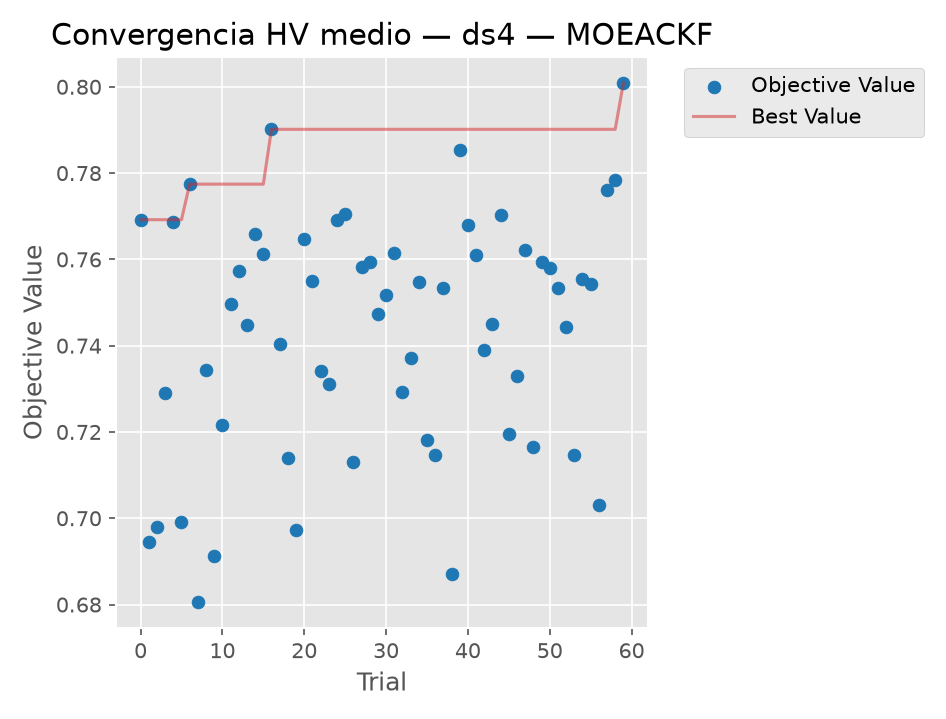
\includegraphics[width=\textwidth]{images/convergencia_MOEACKF_ds4.png}
        \caption{Convergencia del HV medio por \emph{trial} en \texttt{ds4} para MOEA-CKF.}
        \label{fig:ds4_convergencia_ckf}
    \end{subfigure}
    \hfill
    \begin{subfigure}[b]{0.48\textwidth}
        \centering
        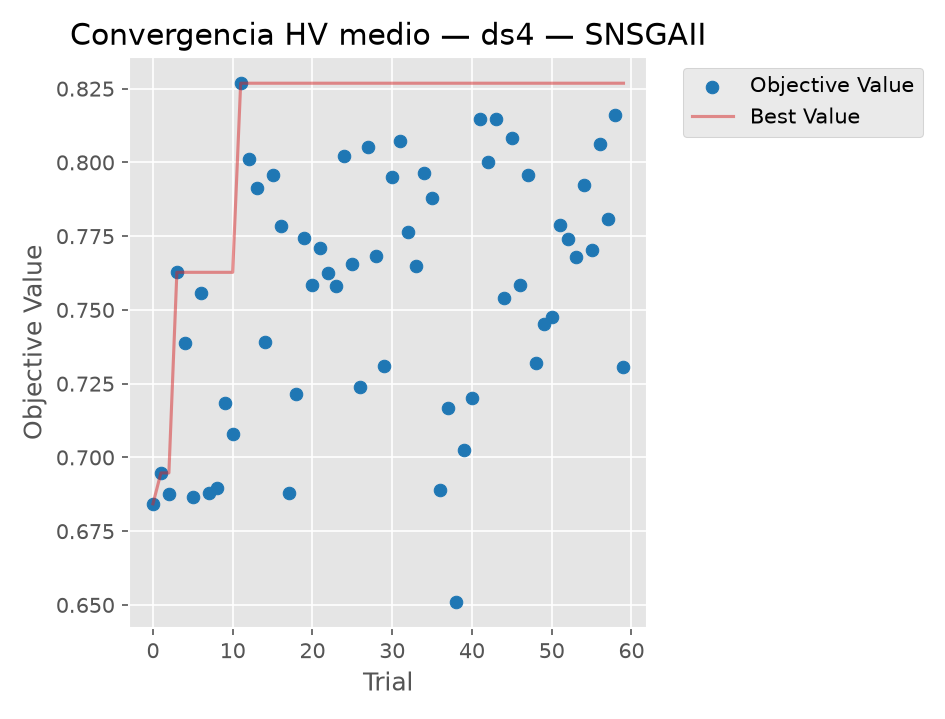
\includegraphics[width=\textwidth]{images/convergencia_SNSGAII_ds4.png}
        \caption{Convergencia del HV medio por \emph{trial} en \texttt{ds4} para S-NSGA-II.}
        \label{fig:ds4_convergencia_nsga}
    \end{subfigure}

    \caption{Comparación de convergencia del hipervolumen entre ambos algoritmos para el Dataset 4.}
    \label{fig:comparacion_hv_ds4}
\end{figure}

El análisis fANOVA en \texttt{ds4} muestra una repartición de importancia más equilibrada y divergente entre algoritmos que en el resto de los datasets: en MOEA-CKF domina \texttt{architecture} (52.7\%), seguido de \texttt{wScale} (32.7\%), mientras que en S-NSGA-II la contribución se reparte principalmente entre \texttt{wScale} (35.9\%) y \texttt{sGap} (35.1\%), con \texttt{sLower} (8.4\%) y \texttt{architecture} (7.9\%) como aportes secundarios. Estos patrones se visualizan en las Figuras~\ref{fig:ds4_fanova_ckf} y~\ref{fig:ds4_fanova_nsga}.

\begin{figure}[htbp]
    \centering

    \begin{subfigure}[b]{0.48\textwidth}
        \centering
        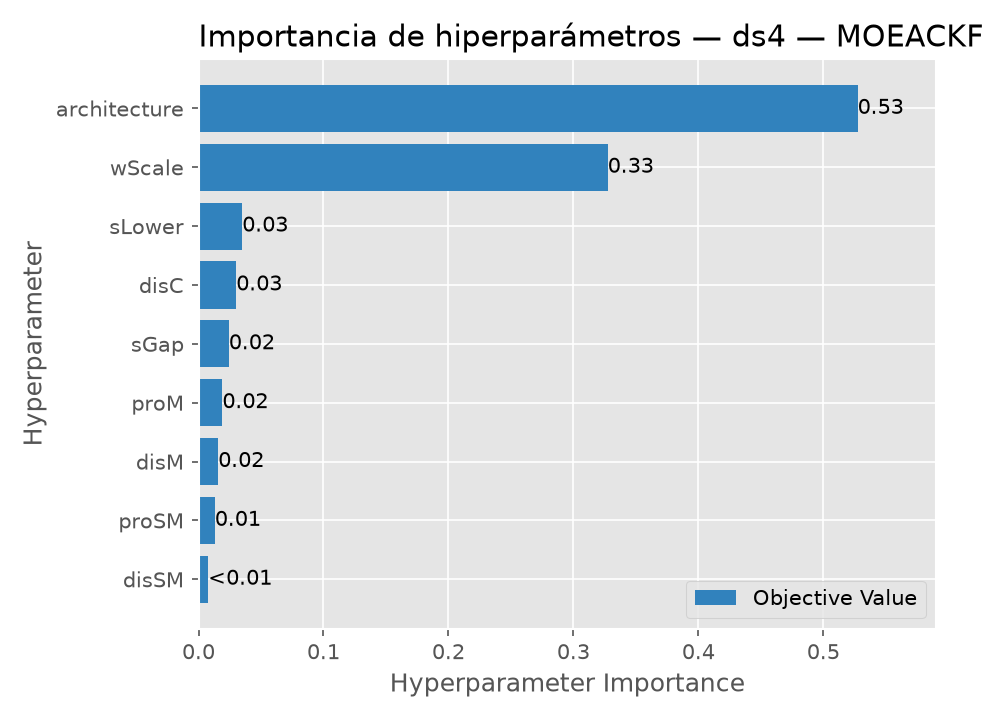
\includegraphics[width=\textwidth]{images/importancia_MOEACKF_ds4.png}
        \caption{Importancia de hiperparámetros (fANOVA) en \texttt{ds4} para MOEA-CKF.}
        \label{fig:ds4_fanova_ckf}
    \end{subfigure}
    \hfill
    \begin{subfigure}[b]{0.48\textwidth}
        \centering
        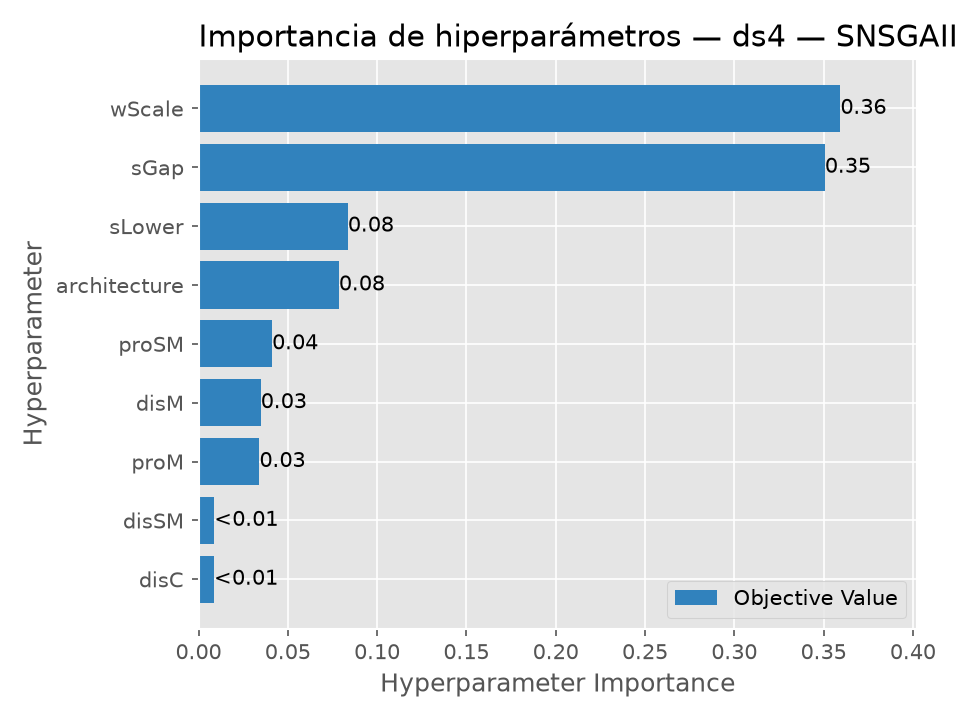
\includegraphics[width=\textwidth]{images/importancia_SNSGAII_ds4.png}
        \caption{Importancia de hiperparámetros (fANOVA) en \texttt{ds4} para S-NSGA-II.}
        \label{fig:ds4_fanova_nsga}
    \end{subfigure}

    \caption{Importancia de hiperparámetros en \texttt{ds4} para ambos algoritmos.}
    \label{fig:importancia_hiper_ds4}
\end{figure}

%-----------------


\providecommand{\Atwelve}{\ensuremath{\hat{A}_{12}}}

\section{Resultados de comparación de algoritmos}
\label{sec:resultados-discusion}

Los resultados y el análisis se organizan en tres experimentos sobre cuatro conjuntos de datos, siguiendo el orden de la Sección~\ref{sec:metodologia-comparacion}. En todos los casos el análisis se realizó por cada dataset, dado que nunca se combinan en una misma prueba estadística. Se reportan los p-valores reportados en cada tabla de los test y su corrección, y se marcaron con \texttt{*} cuando resultaron significativos a $\alpha=0.05$. El veredicto final, obtenido tras aplicar la corrección de Holm-Bonferroni por familias (Sección \ref{subsec:pruebas-estadisticas-correccion}) se menciona en el texto como \textit{tras corrección}. Por último, las tablas reportaron mediana e IQR como estadístico principal, debido a que varios grupos no distribuyen normal, siendo consistente con los tests no paramétricos empleados en todo el documento y la literatura de los algoritmos. Para más detalles sobre los resultados, revisar el repositorio del proyecto en .

\subsection{Comparación de algoritmos en SNN (C++)}
\label{sec:experimento1}

Esta sección compara MOEA-CKF y S-NSGA-II, ambos ejecutados en SNN (C++) sobre el conjunto experimental de referencia ($N=31$ corridas pareadas por semilla), mediante cuatro enfoques: hipervolumen (HV), frentes de Pareto, convergencia y tiempo de cómputo para los cuatro datasets.

\subsubsection{Hipervolumen (HV)}\label{sec:hv}
Los resultados descriptivos se resumen en la Tabla~\ref{tab:hv-summary} para los cuatro datasets. Se muestran la mediana y el IQR. \Atwelve\ se reporta como la fracción de corridas pareadas en las que MOEA-CKF supera a S-NSGA-II (empates cuentan 0.5), de modo que valores por sobre 0.5 favorecen a MOEA-CKF y por debajo de 0.5 favorecen a S-NSGA-II.

\begin{table}[htbp]
\centering
\small
\caption{Resumen del hipervolumen (HV) de MOEA-CKF y S-NSGA-II en los cuatro datasets, $N=31$ corridas pareadas por semilla. El algoritmo con mejor HV estadístico se marca por dataset.}
\label{tab:hv-summary}
\begin{tabular}{cllccc}
\toprule
\textbf{Dataset} & \textbf{MOEA-CKF} & \textbf{S-NSGA-II} & \textbf{$p$ Wilcoxon} & \textbf{$p$ Corregido} & \Atwelve \\
\midrule
1 & \cellcolor{gray!20}$0.8705\ [0.8704,\,0.8721]$ & $0.8459\ [0.7895,\,0.8712]$ & $1.18\times10^{-4}$* & $4.74\times10^{-4}$* & 0.710 \\
2 & \cellcolor{gray!20}$0.9298\ [0.9277,\,0.9319]$ & $0.9278\ [0.9277,\,0.9278]$ & $0.0289$*  & $0.0408$*  & 0.645 \\
3 & $0.7563\ [0.7484,\,0.7634]$ & $0.7520\ [0.7498,\,0.7566]$ & $0.2023$   & $0.2075$   & 0.645 \\
4 & $0.8043\ [0.7936,\,0.8283]$ & \cellcolor{gray!20}$0.8229\ [0.8020,\,0.8418]$ & $0.0051$*  & $0.0254$*  & 0.290 \\
\bottomrule
\end{tabular}
\end{table}

\paragraph{Dataset 1: Statlog Australian}\label{sec:ds1}\label{sec:ds1-hv}
La prueba de Wilcoxon signed-rank arroja una diferencia significativa entre ambos algoritmos, que se mantiene tras la corrección. Esta diferencia se refleja también corrida por corrida: MOEA-CKF superó a S-NSGA-II en 22 de las 31 corridas pareadas (71.0\%), sin empates, lo que corresponde a un efecto a favor de MOEA-CKF.

En este dataset, MOEA-CKF obtiene un HV estadísticamente superior al de S-NSGA-II, con un tamaño de efecto grande. MOEA-CKF es además notablemente más consistente entre corridas: la desviación estándar de S-NSGA-II es cerca de 27 veces la de MOEA-CKF (0.0392 frente a 0.0015), y su corrida más baja queda muy por debajo del mínimo histórico de MOEA-CKF.

\paragraph{Dataset 2: Climate}\label{sec:ds2}\label{sec:ds2-hv}
Existe una diferencia significativa entre ambos algoritmos, que se mantiene tras corrección, aunque de magnitud pequeña: MOEA-CKF superó a S-NSGA-II en 20 de las 31 corridas (64.5\%). La diferencia mediana es de apenas $0.0021$, la más pequeña entre los tres datasets con diferencia significativa, y S-NSGA-II se muestra extremadamente concentrado en torno a su mediana (IQR de solo $0.0001$), mientras que MOEA-CKF exhibe una dispersión bastante mayor (IQR de $0.0042$) pese a tener la mediana más alta.

\paragraph{Dataset 3: Statlog German}\label{sec:ds3}\label{sec:ds3-hv}
No se encuentra una diferencia significativa entre ambos algoritmos, lo que se mantiene tras corrección. MOEA-CKF superó a S-NSGA-II en 20 de las 31 corridas (64.5\%), pero la diferencia mediana es pequeña ($0.0043$) y las medianas de ambos quedan dentro del rango intercuartílico del otro. En conjunto, no hay evidencia suficiente de una diferencia real entre ambos algoritmos en HV para este dataset, pese a que MOEA-CKF gane más seguido corrida por corrida.

\paragraph{Dataset 4: Sonar}\label{sec:ds4}\label{sec:ds4-hv}
Existe una diferencia altamente significativa entre ambos algoritmos, que se mantiene tras corrección. S-NSGA-II superó a MOEA-CKF en 22 de las 31 corridas (71.0\%), lo que corresponde a un efecto a favor de S-NSGA-II.

Este es el único dataset donde se invierte el patrón observado en los tres anteriores: S-NSGA-II supera a MOEA-CKF de forma significativa. Es, además, el dataset con mayor varianza absoluta para ambos algoritmos (60 características), aunque aquí es MOEA-CKF quien muestra la mayor dispersión entre corridas (DE$=0.0326$ frente a $0.0256$ de S-NSGA-II).

\subsubsection{Frentes de Pareto}
\label{sec:fronts}

En la Tabla \ref{tab:fronts-all-datasets} se muestran los resultados de la soluciones de los frentes obtenidos por cada combinación de algoritmo y dataset. La tabla fue construida usando la solución de menor error de entrenamiento por cada una de las 31 corridas.

\begin{table}[htbp]
\centering
\small
\caption{Indicadores de las soluciones de mejor exactitud por corrida para ambos algoritmos en los cuatro datasets en base a la mediana [IQR]. El asterisco (*) indica diferencias estadísticamente significativas, marcando el algoritmo con mejor rendimiento estadístico.}
\label{tab:fronts-all-datasets}

\begin{tabular}{@{}cl|p{3.5cm}p{3.5cm}|cc@{}}
\toprule
\textbf{Dataset} &
\textbf{Indicador} &
\textbf{MOEA-CKF} &
\textbf{S-NSGA-II} &
\textbf{$p$ (Wilcoxon)} &
\Atwelve \\
\midrule

\multirow{3}{*}{1}& Complejidad &
$0.0118\ [0.0088,\,0.0132]$ &
$0.0118\ [0.0074,\,0.0154]$ &
$0.5962$ & 0.581 \\

& Error &
\cellcolor{gray!20}$0.1413\ [0.1395,\,0.1413]$ &
$0.1685\ [0.1395,\,0.2310]$ &
$3.10\times10^{-4}$* & 0.290 \\

& Frente &
$6\ [5,\,7]$ &
$5\ [4,\,7]$ &
$0.4246$ & 0.645 \\
\midrule

\multirow{3}{*}{2}& Complejidad &
$0.0202\ [0.0107,\,0.0339]$ &
\cellcolor{gray!20}$0.0024\ [0.0024,\,0.0048]$ &
$2.86\times10^{-6}$* & 0.919 \\

& Error &
\cellcolor{gray!20}$0.0764\ [0.0741,\,0.0787]$ &
$0.0787\ [0.0787,\,0.0787]$ &
$0.0136$* & 0.306 \\

& Frente &
\cellcolor{gray!20}$5\ [5,\,6]$ &
$3\ [2.5,\,4]$ &
$4.40\times10^{-6}$* & 0.903 \\
\midrule

\multirow{3}{*}{3}& Complejidad &
$0.0120\ [0.0074,\,0.0255]$ &
\cellcolor{gray!20}$0.0028\ [0.0019,\,0.0037]$ &
$3.86\times10^{-6}$* & 0.952 \\

& Error &
$0.2675\ [0.2581,\,0.2762]$ &
$0.2725\ [0.2675,\,0.2750]$ &
$0.1037$ & 0.355 \\

& Frente &
\cellcolor{gray!20}$8\ [5.5,\,10]$ &
$3\ [3,\,4]$ &
$5.26\times10^{-6}$* & 0.935 \\
\midrule

\multirow{3}{*}{4}& Complejidad &
$0.0492\ [0.0167,\,0.0879]$ &
$0.0393\ [0.0333,\,0.0617]$ &
$0.2167$ & 0.548 \\

& Error &
$0.2096\ [0.1856,\,0.2216]$ &
\cellcolor{gray!20}$0.1916\ [0.1707,\,0.2156]$ &
$0.0216$* & 0.677 \\

& Frente &
$10\ [7,\,11.5]$ &
\cellcolor{gray!20}$11\ [9.5,\,14]$ &
$0.0282$* & 0.371 \\

\bottomrule
\end{tabular}
\end{table}

\Atwelve\ se reporta en el mismo sentido que en la Tabla~\ref{tab:hv-summary} (un \Atwelve\ alto significa que MOEA-CKF tiene mayor complejidad o mayor error, no necesariamente que "gane"). En \texttt{ds4}, tanto la diferencia de error como la de tamaño de frente son significativas antes de corrección pero dejan de serlo tras Holm-Bonferroni ($p_{\text{holm}}=0.086$ en ambos casos); se reportan igual en el texto por transparencia, marcando explícitamente que no sobreviven la corrección.

\paragraph{Dataset 1: Statlog Australian}\label{sec:ds1-fronts}
De los tres indicadores, solo la diferencia de error resulta significativa (y se mantiene tras corrección); complejidad y tamaño de frente no muestran diferencias estadísticamente distinguibles entre algoritmos.

El 42.9\% de los puntos del frente combinado de S-NSGA-II están dominados por el de MOEA-CKF, y el 40.0\% en sentido inverso (Figura~\ref{fig:combined-front-ds1}): una cobertura mutua casi simétrica, coherente con que la complejidad y el tamaño de frente no difieran significativamente entre ambos.

\begin{figure}[htbp]
    \centering

    \begin{subfigure}[b]{0.48\textwidth}
        \centering
        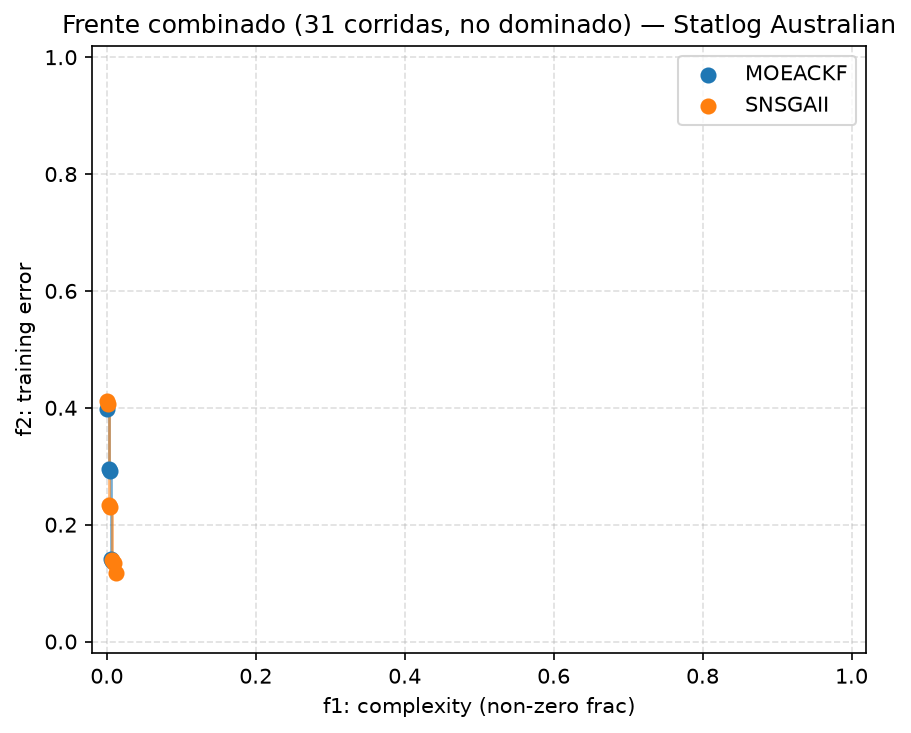
\includegraphics[width=\textwidth]{images/ds1_combined_front.png}
        \caption{Frente combinado (unión no dominada de las 31 corridas) de MOEA-CKF vs.\ S-NSGA-II, dataset 1.}
        \label{fig:combined-front-ds1}
    \end{subfigure}
    \hfill
    \begin{subfigure}[b]{0.48\textwidth}
        \centering
        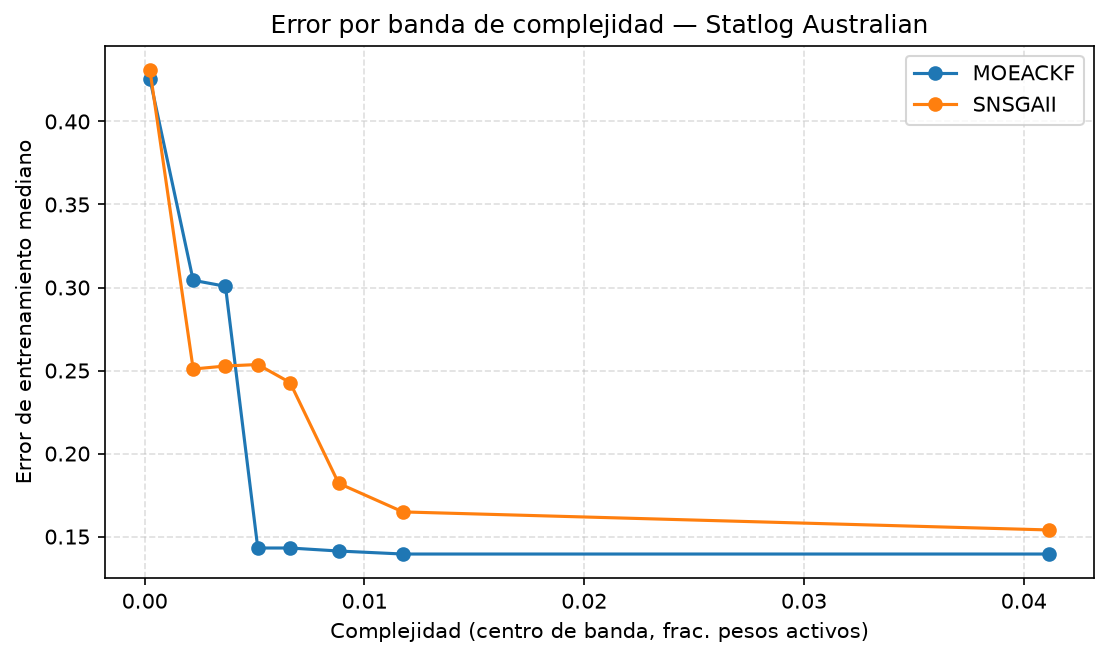
\includegraphics[width=\textwidth]{images/ds1_complexity_bands.png}
        \caption{Error de entrenamiento mediano por banda de complejidad, dataset 1.}
        \label{fig:complexity-bands-ds1}
    \end{subfigure}

    \caption{Frente combinado y bandas de complejidad para dataset 1.}
    \label{fig:frente-bandas-ds1}
\end{figure}

Los deciles sobre el pool de puntos crudos de ambos algoritmos son mostrados en la Figura~\ref{fig:complexity-bands-ds1}. MOEA-CKF obtiene un error mediano menor que S-NSGA-II en la mayoría de las bandas, salvo en una franja de complejidad baja-media ($\sim0.0015$–$0.0044$), donde S-NSGA-II es mejor (p.\,ej.\ $0.251$ vs.\ $0.304$). Ninguno de los dos algoritmos concentra su masa de forma marcadamente distinta de la del otro en este dataset, consistente con la ausencia de diferencia significativa en complejidad y tamaño de frente.

\paragraph{Dataset 2: Climate.}\label{sec:ds2-fronts}
Complejidad y tamaño de frente son significativos y se mantienen tras corrección; el error de las mejores redes también es significativo, aunque con una diferencia mediana pequeña ($0.0764$ vs.\ $0.0787$). En cuanto a complejidad, S-NSGA-II encuentra redes de mejor exactitud más pequeñas que MOEA-CKF con $\Atwelve=0.919$, logrando un error de entrenamiento apenas distinto (y menor) que el de MOEA-CKF. Este último necesita, en cambio, redes más densas y más variables, y retiene además un frente más grande (mediana 5 frente a 3). La cobertura de los frentes combinados no es simétrica: el 33.3\% de los puntos del frente de S-NSGA-II están cubiertos por el de MOEA-CKF, y el 42.9\% en sentido inverso (Figura~\ref{fig:combined-front-ds2}).

\begin{figure}[htbp]
    \centering

    \begin{subfigure}[b]{0.48\textwidth}
        \centering
        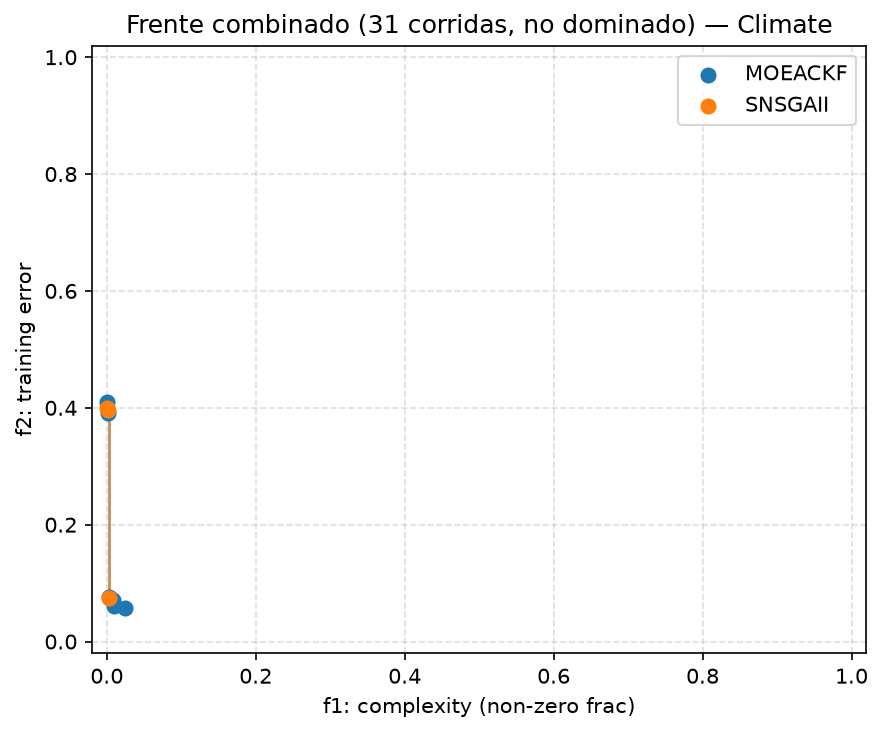
\includegraphics[width=\textwidth]{images/ds2_combined_front.png}
        \caption{Frente combinado (unión no dominada de las 31 corridas) de MOEA-CKF vs.\ S-NSGA-II, dataset 2.}
        \label{fig:combined-front-ds2}
    \end{subfigure}
    \hfill
    \begin{subfigure}[b]{0.48\textwidth}
        \centering
        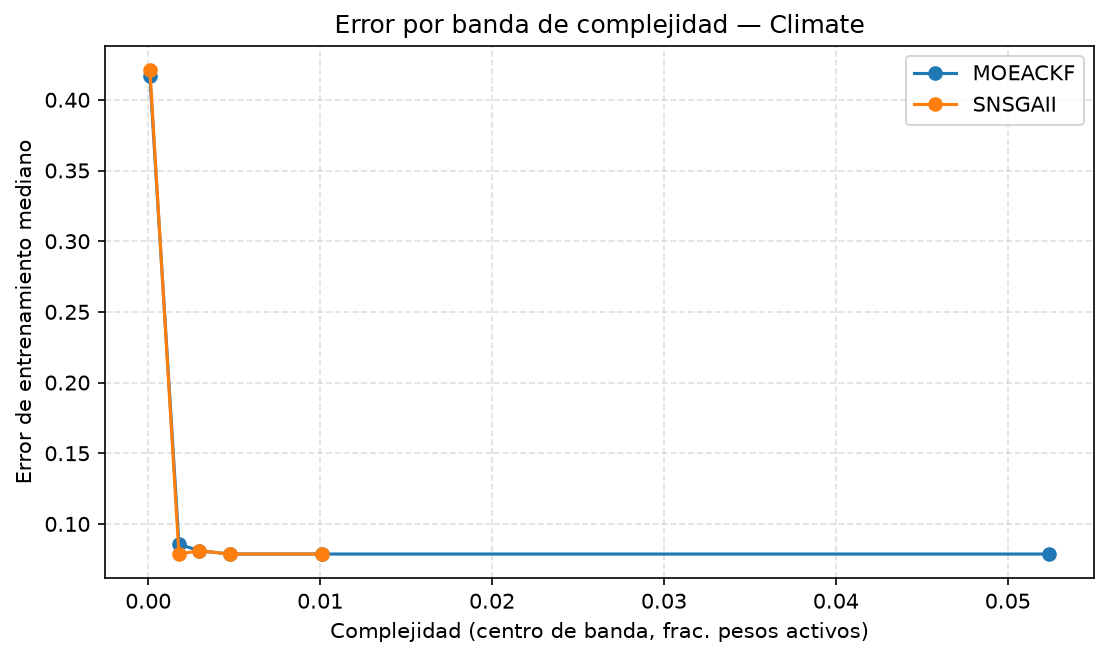
\includegraphics[width=\textwidth]{images/ds2_complexity_bands.png}
        \caption{Error de entrenamiento mediano por banda de complejidad, dataset 2.}
        \label{fig:complexity-bands-ds2}
    \end{subfigure}

    \caption{Frente combinado y bandas de complejidad para dataset 2.}
    \label{fig:frente-bandas-ds2}
\end{figure}

Los deciles sobre el pool de puntos crudos de ambos algoritmos son mostrados en la Figura \ref{fig:complexity-bands-ds2}. S-NSGA-II prácticamente no tiene puntos más allá de la banda de complejidad $0.0060$–$0.0143$ (un solo punto de 31 corridas cae ahí, y ninguno en la banda superior): sus corridas concentran casi toda su masa en las bandas de menor complejidad, mientras que MOEA-CKF se extiende hasta $\sim0.09$. En la banda de complejidad más baja distinta de cero, MOEA-CKF tiene un error mediano algo mayor que S-NSGA-II ($0.0856$ vs.\ $0.0787$); de ahí en adelante ambos convergen al mismo error de $0.0787$, de modo que la ventaja de S-NSGA-II en esta zona es sobre todo de complejidad, no de error.

\paragraph{Dataset 3: Statlog German.}\label{sec:ds3-fronts}
Complejidad y tamaño de frente son significativos y se mantienen tras corrección; la diferencia de error, en cambio, no es significativa. S-NSGA-II incurre en menos complejidad en sus mejores redes, con un error estadísticamente indistinguible del de MOEA-CKF, y retiene frentes sustancialmente más grandes.

Como se observa en la Figura~\ref{fig:combined-front-ds3}, el $20.0\%$ de las soluciones del frente combinado de S-NSGA-II son dominadas por alguna solución de MOEA-CKF. De manera recíproca, MOEA-CKF domina el $50.0\%$ de las soluciones de S-NSGA-II: pese a que MOEA-CKF tiene el doble de puntos en su frente combinado, es su propio frente el más cubierto por el del otro algoritmo, no al revés.

% Este comportamiento sugiere que ninguno de los algoritmos domina de forma concluyente al otro en toda la región de interés. Más bien, ambos conservan soluciones competitivas en distintas zonas del frente de Pareto, aunque S-NSGA-II presenta una mayor capacidad para generar alternativas no dominadas y, con ello, una representación más extensa entre complejidad estructural y error de clasificación.

\begin{figure}[htbp]
    \centering

    \begin{subfigure}[b]{0.48\textwidth}
        \centering
        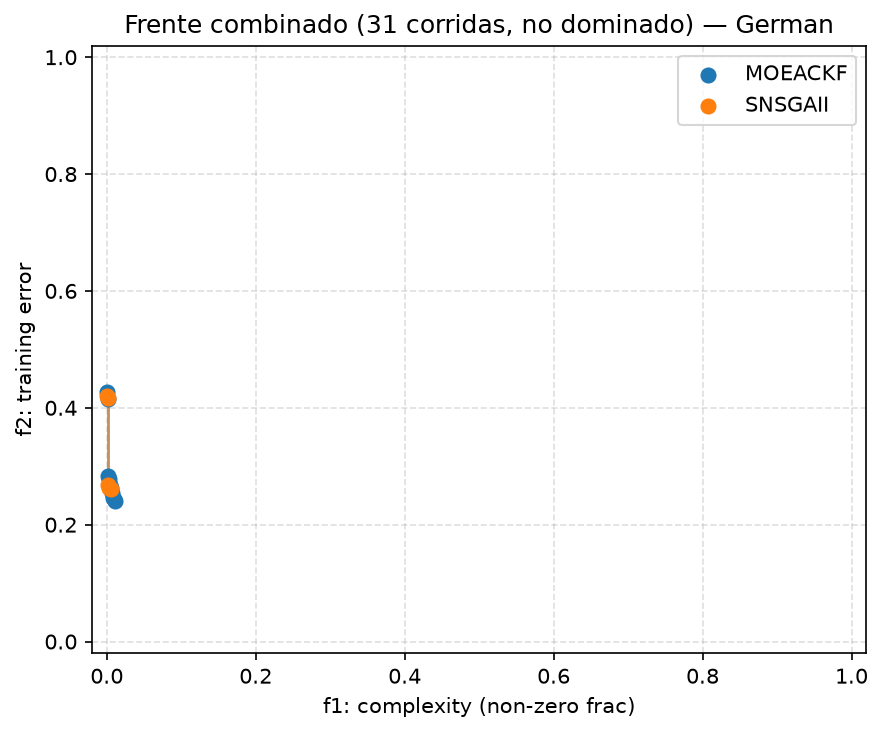
\includegraphics[width=\textwidth]{images/ds3_combined_front.png}
        \caption{Frente combinado (unión no dominada de las 31 corridas) de MOEA-CKF vs.\ S-NSGA-II, dataset 3.}
        \label{fig:combined-front-ds3}
    \end{subfigure}
    \hfill
    \begin{subfigure}[b]{0.48\textwidth}
        \centering
        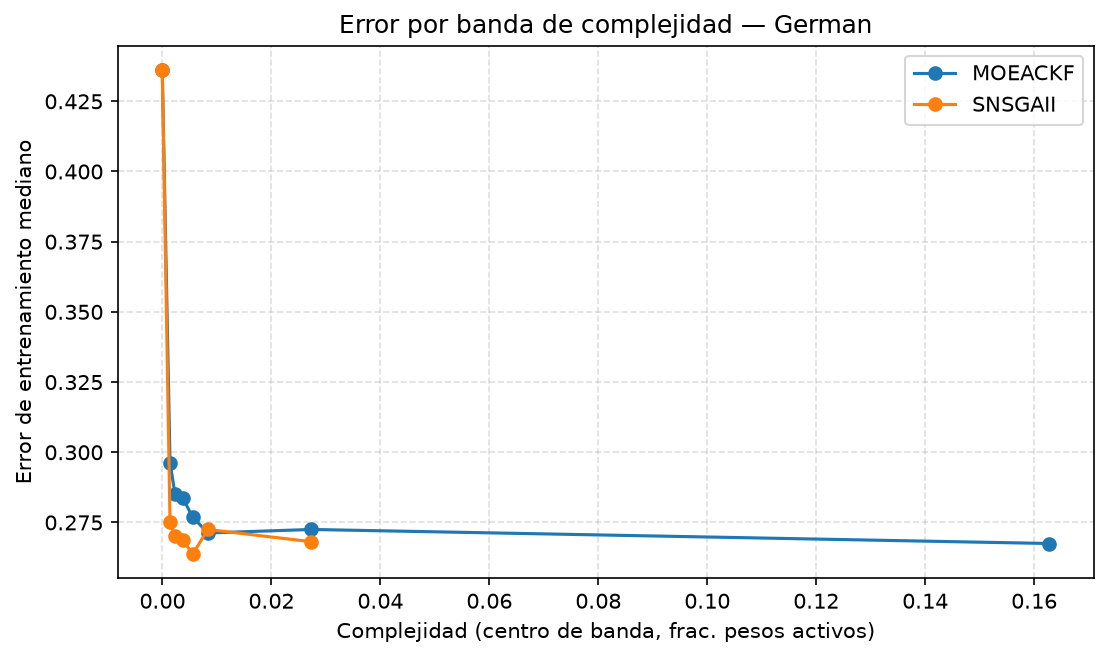
\includegraphics[width=\textwidth]{images/ds3_complexity_bands.png}
        \caption{Error de entrenamiento mediano por banda de complejidad, dataset 3.}
        \label{fig:complexity-bands-ds3}
    \end{subfigure}

    \caption{Frente combinado y bandas de complejidad para dataset 3.}
    \label{fig:frente-bandas-ds3}
\end{figure}

La distribución del error según bandas de complejidad se presenta en la Figura~\ref{fig:complexity-bands-ds3}. En la banda de complejidad nula ambos algoritmos son prácticamente idénticos. Desde $\approx0.001$ y hasta $\approx0.0065$, S-NSGA-II obtiene errores consistentemente menores que MOEA-CKF, aunque con muestras cada vez más pequeñas a medida que sube la complejidad; de ahí en adelante los pocos puntos restantes de S-NSGA-II (2–3 por banda) quedan cerca de MOEA-CKF, y solo este último alcanza la banda de mayor complejidad ($>0.0445$, 37 puntos).

\paragraph{Dataset 4: Sonar}\label{sec:ds4-fronts}

De los tres indicadores, complejidad no resulta significativa; error y tamaño de frente sí lo son antes de corrección, pero ninguno de los dos sobrevive Holm-Bonferroni (ver nota bajo la Tabla~\ref{tab:fronts-all-datasets}). Con esa salvedad, S-NSGA-II tiende a redes con menor error y frentes algo más grandes que MOEA-CKF.

\begin{figure}[htbp]
    \centering

    \begin{subfigure}[b]{0.48\textwidth}
        \centering
        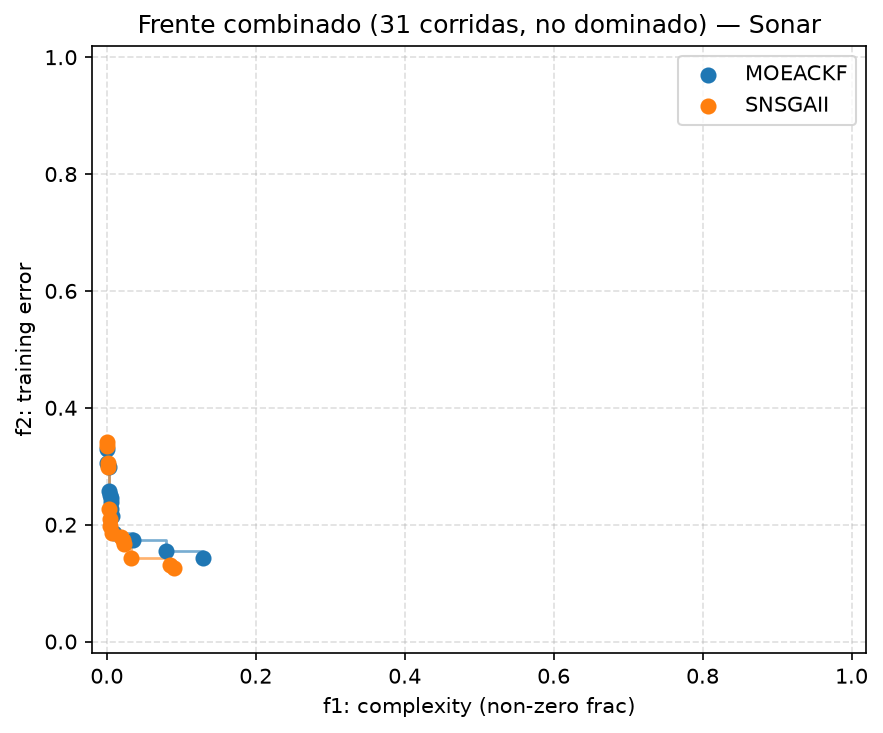
\includegraphics[width=\textwidth]{images/ds4_combined_front.png}
        \caption{Frente combinado (unión no dominada de las 31 corridas) de MOEA-CKF vs.\ S-NSGA-II, dataset 4.}
        \label{fig:combined-front-ds4}
    \end{subfigure}
    \hfill
    \begin{subfigure}[b]{0.48\textwidth}
        \centering
        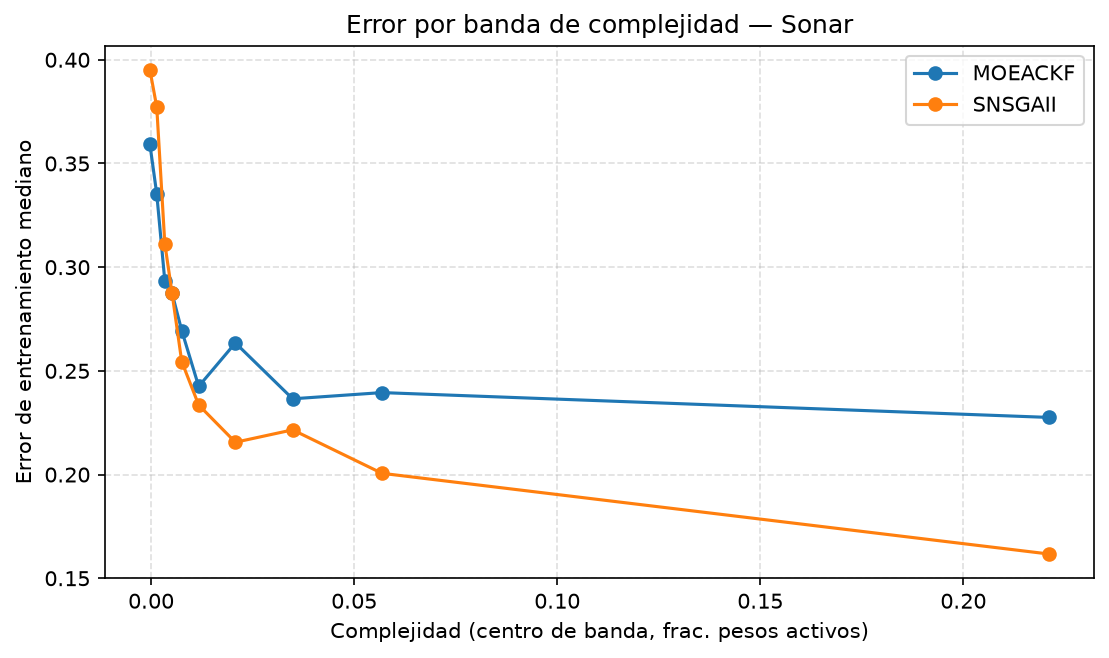
\includegraphics[width=\textwidth]{images/ds4_complexity_bands.png}
        \caption{Error de entrenamiento mediano por banda de complejidad, dataset 4.}
        \label{fig:complexity-bands-ds4}
    \end{subfigure}

    \caption{Frente combinado y bandas de complejidad para dataset 4.}
    \label{fig:frente-bandas-ds4}
\end{figure}

El 84.6\% de las soluciones del frente combinado de MOEA-CKF (13 puntos) son dominadas por alguna solución del frente de S-NSGA-II (14 puntos). Al revés, solo el 21.4\% de las soluciones de S-NSGA-II son dominadas por alguna solución de MOEA-CKF, siendo el resultado más asimétrico de los cuatro datasets, y en sentido opuesto al observado en \texttt{ds3} (Figura~\ref{fig:combined-front-ds4}).

S-NSGA-II presenta un error menor que MOEA-CKF en la mayor parte del rango de complejidad (Figura \ref{fig:complexity-bands-ds4}), con MOEA-CKF por delante únicamente en las tres bandas de menor complejidad (hasta $\approx0.0044$); a partir de ahí S-NSGA-II domina de forma sostenida hasta la banda de mayor complejidad, donde además concentra la muestra más grande de puntos (59 frente a 9 de MOEA-CKF). La ventaja de S-NSGA-II en este dataset es amplia y se concentra en la región de complejidad media a alta, mientras que MOEA-CKF solo es preferible en el extremo más esparso.

\subsubsection{Convergencia}\label{sec:convergencia}

\begin{figure}[htbp]
    \centering

    % Fila 1
    \begin{subfigure}[b]{0.48\textwidth}
        \centering
        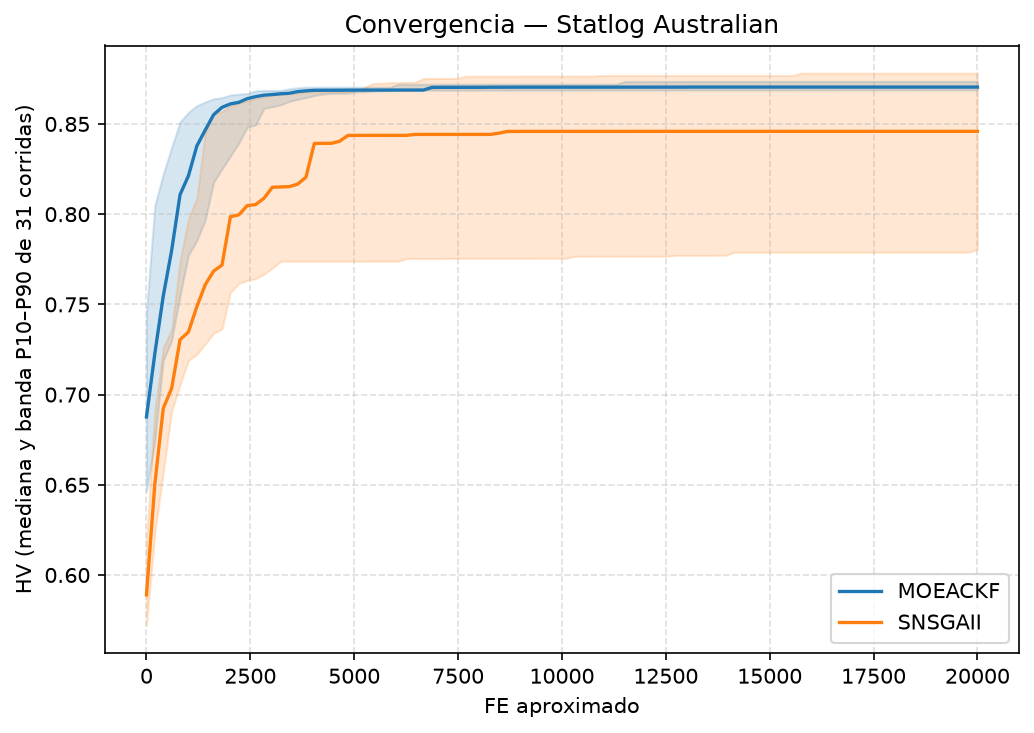
\includegraphics[width=\textwidth]{images/ds1_convergence.png}
        \caption{Curva de convergencia, dataset 1.}
        \label{fig:convergence-ds1}
    \end{subfigure}
    \hfill
    \begin{subfigure}[b]{0.48\textwidth}
        \centering
        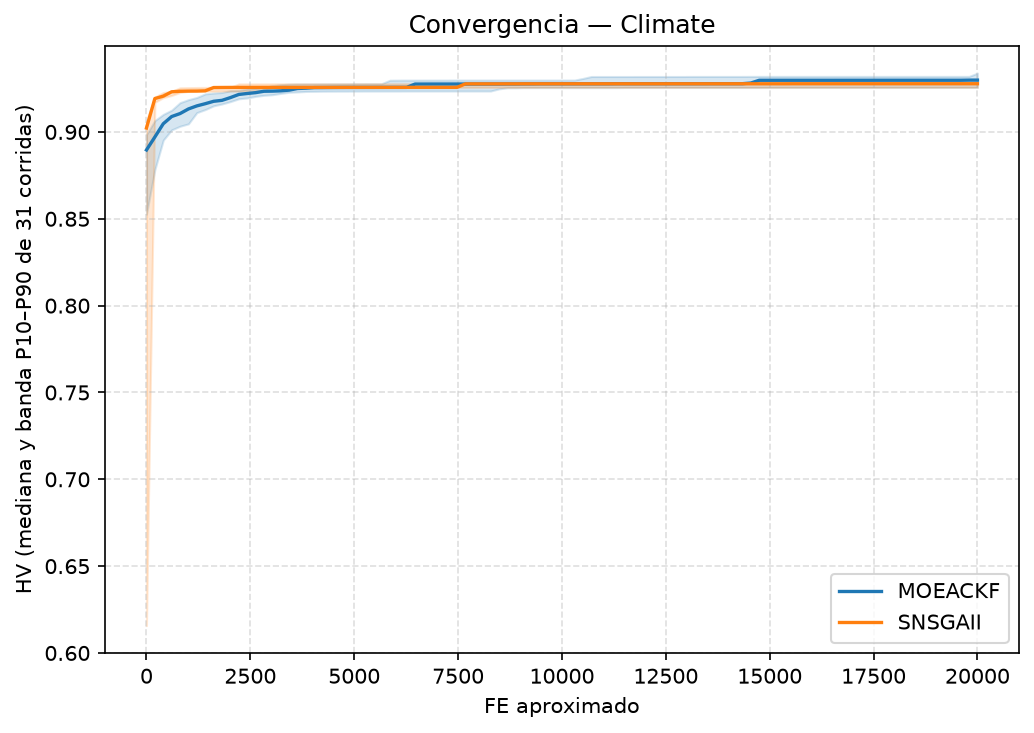
\includegraphics[width=\textwidth]{images/ds2_convergence.png}
        \caption{Curva de convergencia, dataset 2.}
        \label{fig:convergence-ds2}
    \end{subfigure}

    \vspace{0.5cm}

    % Fila 2
    \begin{subfigure}[b]{0.48\textwidth}
        \centering
        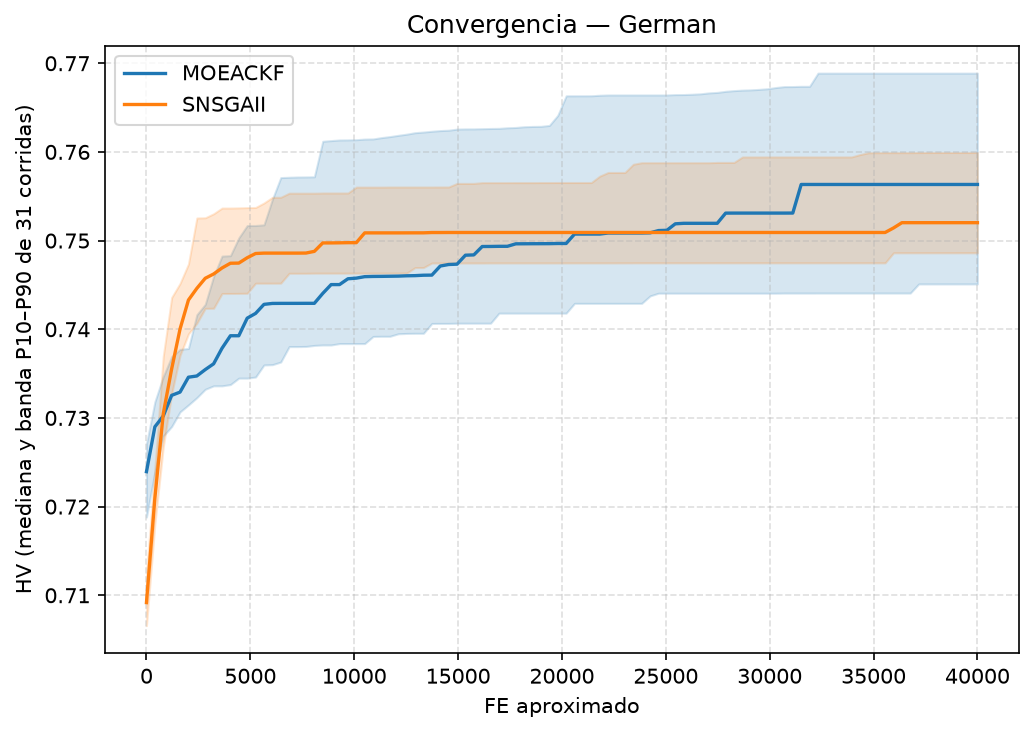
\includegraphics[width=\textwidth]{images/ds3_convergence.png}
        \caption{Curva de convergencia dataset 3.}
        \label{fig:convergence-ds3}
    \end{subfigure}
    \hfill
    \begin{subfigure}[b]{0.48\textwidth}
        \centering
        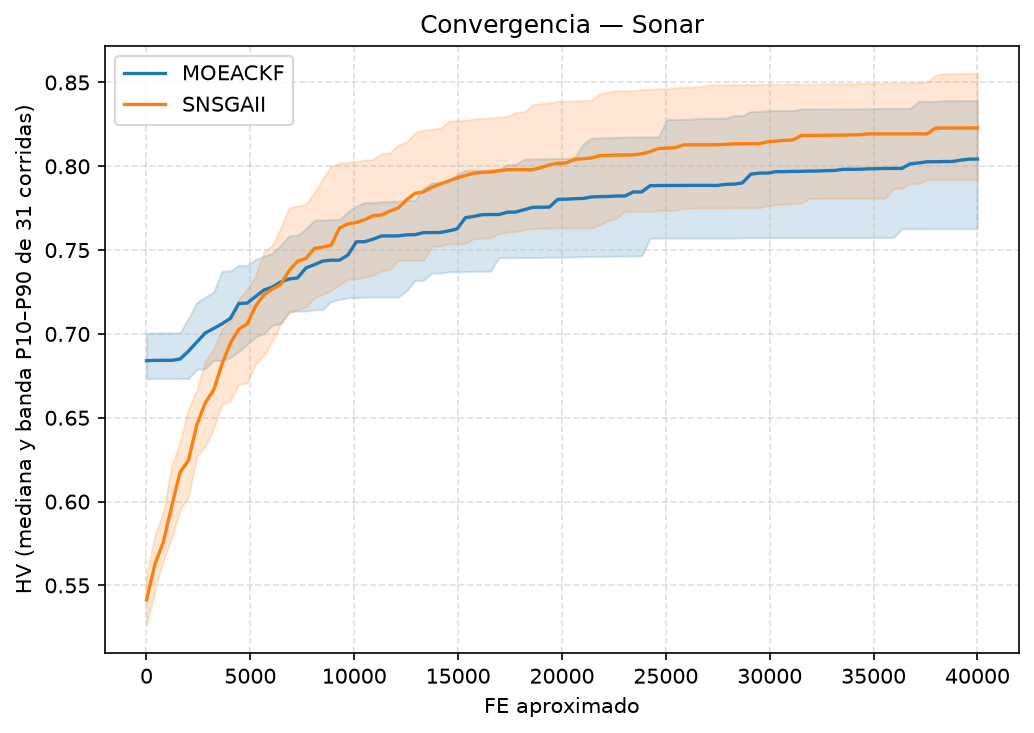
\includegraphics[width=\textwidth]{images/ds4_convergence.png}
        \caption{Curva de convergencia dataset 4.}
        \label{fig:convergence-ds4}
    \end{subfigure}

    \caption{Comparación de las curvas de convergencia para los cuatro datasets.}
    \label{fig:cuadrante}
\end{figure}

\paragraph{Dataset 1: Statlog Australian}\label{sec:ds1-convergencia}

Según la Figura~\ref{fig:convergence-ds1}, MOEA-CKF converge más rápido al comienzo: sube abruptamente y se estabiliza cerca de $\text{FE}\approx3000$-$5000$ en $\text{HV}\approx0.87$. S-NSGA-II, en cambio, arranca más bajo y asciende de forma escalonada, sin llegar a superar el \textit{plateau} de MOEA-CKF y terminando establemente por debajo, en $\text{HV}\approx0.845$.

En las 31 corridas, MOEA-CKF alcanza el 95\% de su propio HV final antes que S-NSGA-II, siendo la diferencia significativa tras corrección. MOEA-CKF en este dataset es más rápido para llegar a su techo como y el que alcanza el techo más alto (Sección~\ref{sec:ds1-hv}).

\paragraph{Dataset 2: Climate}\label{sec:ds2-convergencia}

En las 31 corridas de \textbf{ambos} algoritmos, la población inicial (generación 0) ya alcanza el 90\% del HV final en la mediana, sin diferencia significativa entre algoritmos en ese umbral. Al 95\% sí aparece una diferencia pequeña pero significativa tras corrección: S-NSGA-II llega más consistentemente ya en $\text{FE}\approx0$. 
% (mediana y IQR completos en 0), mientras que el IQR superior de MOEA-CKF llega hasta FE$\approx127$, es decir, unas pocas corridas de MOEA-CKF tardan algo más en estabilizarse. Esto es consistente con que Climate sea, para ambos algoritmos, un problema comparativamente \textit{saturado}: el margen de mejora sobre la población inicial es pequeño, de modo que la velocidad de convergencia aquí mide más bien qué tan rápido se estabiliza la búsqueda que una carrera real de optimización.

\paragraph{Dataset 3: Statlog German}\label{sec:ds3-convergencia}

La curva (Figura~\ref{fig:convergence-ds3}) muestra a S-NSGA-II arrancando más bajo ($\sim0.709$) y ascendiendo con pendiente más pronunciada al inicio, cruzando a MOEA-CKF cerca de $\text{FE}\approx10000$ y manteniéndose por encima de él en la mayor parte del presupuesto restante, aunque con una banda de incertidumbre de MOEA-CKF que se ensancha hacia el final y llega a solaparse con la de S-NSGA-II.

A diferencia de los otros tres datasets, la diferencia de velocidad de convergencia al 95\% no es significativa aquí, aunque la mediana de MOEA-CKF sigue siendo menor que la de S-NSGA-II. Al umbral del 90\% ambos algoritmos alcanzan ese nivel ya en la generación 0 en las 31 corridas, por lo que no hay evidencia de diferencia en ese umbral más laxo.

\paragraph{Dataset 4: Sonar}\label{sec:ds4-convergencia}

Según la Figura~\ref{fig:convergence-ds4}, S-NSGA-II se mantiene por encima de MOEA-CKF durante casi todo el presupuesto y asciende de forma más pronunciada desde el inicio, mientras que MOEA-CKF parte más alto en las primeras evaluaciones pero avanza con mayor lentitud y termina por debajo, sin llegar a aplanarse del todo cerca de $\text{FE}=40000$.

La diferencia de velocidad de convergencia al 95\% no resulta significativa en este dataset, pese a que S-NSGA-II obtiene el HV final más alto (Sección~\ref{sec:ds4-hv}): ambos algoritmos tardan una fracción comparable de su presupuesto en estabilizarse (medianas de $14212$ y $12632$ FE, respectivamente). Al umbral del 90\% sí aparece una diferencia, con MOEA-CKF llegando algo antes.

\subsubsection{Tiempo de cómputo}\label{sec:tiempo-referencia}

Cada algoritmo usa aquí los hiperparámetros que encontró en su propia búsqueda bayesiana, incluyendo el codificador (Poisson o TTFS) y el nivel de esparsidad, por lo que el tiempo medido refleja el costo real incurrido en el experimento principal.

\begin{table}[htbp]
\centering
\small
\caption{Tiempo de ejecución de MOEA-CKF y S-NSGA-II en el conjunto de referencia, $N=31$ corridas pareadas por semilla. Se muestra la mediana [IQR]. El asterisco (*) indica diferencias estadísticamente significativas según la prueba de Wilcoxon. El algoritmo más rápido está destacado.}
\label{tab:time-referencia}
\begin{tabular}{ccccc}
\toprule
\textbf{Dataset} &
\textbf{MOEA-CKF} &
\textbf{S-NSGA-II} &
\textbf{$p$ (Wilcoxon)} &
\Atwelve \\
\midrule

1 &
$275.4\ [259.7,\,284.3]$ s &
\cellcolor{gray!20}$159.5\ [155.3,\,165.3]$ s &
$9.31\times10^{-10}$* & 1.000 \\

2 &
\cellcolor{gray!20}$188.1\ [174.4,\,213.1]$ s &
$223.4\ [204.0,\,243.8]$ s &
$4.53\times10^{-4}$* & 0.226 \\

3 &
\cellcolor{gray!20}$627.8\ [578.8,\,664.6]$ s &
$1026.0\ [995.4,\,1063.0]$ s &
$9.31\times10^{-10}$* & 0.000 \\

4 &
$477.4\ [427.4,\,640.3]$ s &
\cellcolor{gray!20}$167.4\ [166.5,\,170.9]$ s &
$9.31\times10^{-10}$* & 1.000 \\

\bottomrule
\end{tabular}
\end{table}

Las cuatro comparaciones son significativas, tanto antes como después de la corrección por comparaciones múltiples (Tabla~\ref{tab:time-referencia}), y el algoritmo más rápido cambia según el dataset: S-NSGA-II es más rápido en \texttt{ds1} y \texttt{ds4}, mientras que MOEA-CKF lo es en \texttt{ds2} y \texttt{ds3}. Este patrón coincide exactamente con el codificador que cada algoritmo seleccionó en su propia búsqueda de hiperparámetros (Tabla~\ref{tab:hv_por_dataset_resultados}): en \texttt{ds2} y \texttt{ds3}, donde MOEA-CKF gana con TTFS y S-NSGA-II con Poisson, es MOEA-CKF quien resulta más rápido; en \texttt{ds1}, donde los codificadores están invertidos (MOEA-CKF con Poisson, S-NSGA-II con TTFS), es S-NSGA-II quien gana. La única excepción aparente es \texttt{ds4}, donde ambos algoritmos comparten codificador TTFS y, aun así, S-NSGA-II es sustancialmente más rápido (con la mayor brecha relativa de las cuatro, $\Atwelve=1.000$, sin una sola corrida en sentido contrario), lo que aísla un costo algorítmico propio de MOEA-CKF independiente del codificador.

\subsection{Plataforma SNN (C++) vs.\ ANN (MATLAB)}
\label{sec:experimento2}

Esta sección compara cada algoritmo entre su implementación SNN (C++) sobre el conjunto experimental de referencia y la implementación ANN original de PlatEMO/MATLAB, para los cuatro datasets.

\paragraph{Dataset 1: Statlog Australian}
\label{sec:ds1-plataforma}
Las seis comparaciones (Tablas~\ref{tab:platform-MOEA-CKF-ds1} y \ref{tab:platform-S-NSGA-II-ds1}) son significativas y se mantienen tras corrección. La implementación original en ANN (MATLAB) supera de forma consistente a la SNN en HV, con un error de entrenamiento menor para ambos algoritmos y una brecha de error de $\sim0.02$ en MOEA-CKF y $\sim0.06$ en S-NSGA-II. Las redes de menor error en ANN también son más densas que las SNN en ambos algoritmos, con la brecha de complejidad más marcada en S-NSGA-II (impulsada por algunas corridas en MATLAB que alcanzan redes casi densas).

\begin{table}[htbp]
\centering
\small
\caption{MOEA-CKF: SNN vs.\ ANN (MATLAB), dataset 1.}
\label{tab:platform-MOEA-CKF-ds1}
\begin{tabular}{@{}l|p{3.2cm}p{3.2cm}|cc@{}}
\toprule
\textbf{Indicador} & \textbf{MOEA-CKF: SNN} & \textbf{MOEA-CKF: ANN} &
  \textbf{$p$ (Mann-Whitney)} & \Atwelve \\
\midrule
HV &  $0.8705\ [0.8704,\,0.8721]$ &  \cellcolor{gray!20}$0.8891\ [0.8891,\,0.8907]$ &
  $1.37\times10^{-11}$* & 0.000 \\
Complejidad &  \cellcolor{gray!20}$0.0118\ [0.0088,\,0.0132]$ &  $0.0203\ [0.0140,\,0.0390]$ &
  $1.99\times10^{-6}$* & 0.149 \\
Error &  $0.1413\ [0.1395,\,0.1413]$ &  \cellcolor{gray!20}$0.1196\ [0.1178,\,0.1196]$ &
  $5.26\times10^{-12}$* & 1.000 \\
\bottomrule
\end{tabular}

\bigskip
\centering
\caption{S-NSGA-II: SNN vs.\ ANN (MATLAB), dataset 1.}
\label{tab:platform-S-NSGA-II-ds1}
\begin{tabular}{@{}l|p{3.2cm}p{3.2cm}|cc@{}}
\toprule
\textbf{Indicador} & \textbf{S-NSGA-II: SNN} & \textbf{S-NSGA-II: ANN} &
  \textbf{$p$ (Mann-Whitney)} & \Atwelve \\
\midrule
HV &  $0.8459\ [0.7895,\,0.8712]$ &  \cellcolor{gray!20}$0.8972\ [0.8948,\,0.8979]$ &
  $1.54\times10^{-11}$* & 0.001 \\
Complejidad &  \cellcolor{gray!20}$0.0118\ [0.0074,\,0.0154]$ &  $0.0265\ [0.0265,\,0.1256]$ &
  $4.88\times10^{-11}$* & 0.020 \\
Error &  $0.1685\ [0.1395,\,0.2310]$ &  \cellcolor{gray!20}$0.1105\ [0.1096,\,0.1123]$ &
  $1.08\times10^{-11}$* & 1.000 \\
\bottomrule
\end{tabular}
\end{table}

\paragraph{Dataset 2: Climate}
\label{sec:ds2-plataforma}
Todas las comparaciones son significativas tras corrección (Tablas~\ref{tab:platform-MOEA-CKF-ds2} y \ref{tab:platform-S-NSGA-II-ds2}). La brecha ANN-SNN en HV es la más grande de los cuatro datasets para ambos algoritmos, y también lo es en error de entrenamiento. La complejidad, en cambio, diverge fuertemente según el algoritmo: para MOEA-CKF las redes ANN son más densas que las de SNN, mientras que para S-NSGA-II las redes ANN de menor error son casi completamente densas frente a las redes SNN. Para llegar a su menor error, S-NSGA-II-ANN necesita casi todos los pesos activos, mientras que en SNN logra un error de entrenamiento bastante mayor con una fracción minúscula de la red.

\begin{table}[htbp]
\centering
\small
\caption{MOEA-CKF: SNN vs.\ ANN (MATLAB), dataset 2.}
\label{tab:platform-MOEA-CKF-ds2}
\begin{tabular}{@{}l|p{3.2cm}p{3.2cm}|cc@{}}
\toprule
\textbf{Indicador} & \textbf{MOEA-CKF: SNN} & \textbf{MOEA-CKF: ANN} &
  \textbf{$p$ (Mann-Whitney)} & \Atwelve \\
\midrule
HV &  $0.9298\ [0.9277,\,0.9319]$ &  \cellcolor{gray!20}$0.9767\ [0.9747,\,0.9770]$ &
  $1.40\times10^{-11}$* & 0.000 \\
Complejidad &  \cellcolor{gray!20}$0.0202\ [0.0107,\,0.0339]$ &  $0.0487\ [0.0399,\,0.0662]$ &
  $1.88\times10^{-7}$* & 0.114 \\
Error &  $0.0764\ [0.0741,\,0.0787]$ &  \cellcolor{gray!20}$0.0232\ [0.0232,\,0.0255]$ &
  $7.31\times10^{-12}$* & 1.000 \\
\bottomrule
\end{tabular}

\bigskip
\centering
\caption{S-NSGA-II: SNN vs.\ ANN (MATLAB), dataset 2.}
\label{tab:platform-S-NSGA-II-ds2}
\begin{tabular}{@{}l|p{3.2cm}p{3.2cm}|cc@{}}
\toprule
\textbf{Indicador} & \textbf{S-NSGA-II: SNN} & \textbf{S-NSGA-II: ANN} &
  \textbf{$p$ (Mann-Whitney)} & \Atwelve \\
\midrule
HV &  $0.9278\ [0.9277,\,0.9278]$ &  \cellcolor{gray!20}$0.9477\ [0.9440,\,0.9539]$ &
  $1.39\times10^{-11}$* & 0.000 \\
Complejidad &  \cellcolor{gray!20}$0.0024\ [0.0024,\,0.0048]$ &  $0.9114\ [0.7316,\,0.9601]$ &
  $5.12\times10^{-12}$* & 0.000 \\
Error &  $0.0787\ [0.0787,\,0.0787]$ &  \cellcolor{gray!20}$0.0347\ [0.0301,\,0.0370]$ &
  $3.04\times10^{-12}$* & 1.000 \\
\bottomrule
\end{tabular}
\end{table}

\paragraph{Dataset 3: Statlog German}
\label{sec:ds3-plataforma}
Todas las comparaciones son significativas tras corrección (Tablas~\ref{tab:platform-MOEA-CKF-ds3} y \ref{tab:platform-S-NSGA-II-ds3}): las redes ANN de MOEA-CKF son más densas que las SNN, mientras que las redes ANN de S-NSGA-II vuelven a ser casi totalmente densas frente a redes SNN mucho más esparsas.

\begin{table}[htbp]
\centering
\small
\caption{MOEA-CKF: SNN vs.\ ANN (MATLAB), dataset 3.}
\label{tab:platform-MOEA-CKF-ds3}
\begin{tabular}{@{}l|p{3.2cm}p{3.2cm}|cc@{}}
\toprule
\textbf{Indicador} & \textbf{MOEA-CKF: SNN} & \textbf{MOEA-CKF: ANN} &
  \textbf{$p$ (Mann-Whitney)} & \Atwelve \\
\midrule
HV &  $0.7563\ [0.7484,\,0.7634]$ &  \cellcolor{gray!20}$0.8098\ [0.8082,\,0.8111]$ &
  $1.40\times10^{-11}$* & 0.000 \\
Complejidad &  \cellcolor{gray!20}$0.0120\ [0.0074,\,0.0255]$ &  $0.0413\ [0.0375,\,0.0644]$ &
  $1.80\times10^{-6}$* & 0.147 \\
Error &  $0.2675\ [0.2581,\,0.2763]$ &  \cellcolor{gray!20}$0.2075\ [0.2063,\,0.2094]$ &
  $1.24\times10^{-11}$* & 1.000 \\
\bottomrule
\end{tabular}

\bigskip
\centering
\caption{S-NSGA-II: SNN vs.\ ANN (MATLAB), dataset 3.}
\label{tab:platform-S-NSGA-II-ds3}
\begin{tabular}{@{}l|p{3.2cm}p{3.2cm}|cc@{}}
\toprule
\textbf{Indicador} & \textbf{S-NSGA-II: SNN} & \textbf{S-NSGA-II: ANN} &
  \textbf{$p$ (Mann-Whitney)} & \Atwelve \\
\midrule
HV &  $0.7520\ [0.7498,\,0.7566]$ &  \cellcolor{gray!20}$0.8119\ [0.8098,\,0.8132]$ &
  $1.40\times10^{-11}$* & 0.000 \\
Complejidad &  \cellcolor{gray!20}$0.0028\ [0.0019,\,0.0037]$ &  $0.8751\ [0.3506,\,0.9942]$ &
  $1.01\times10^{-11}$* & 0.000 \\
Error &  $0.2725\ [0.2675,\,0.2750]$ &  \cellcolor{gray!20}$0.2025\ [0.1994,\,0.2038]$ &
  $1.27\times10^{-11}$* & 1.000 \\
\bottomrule
\end{tabular}
\end{table}

\paragraph{Dataset 4: Sonar}
\label{sec:ds4-plataforma}

Cinco de las seis comparaciones son significativas tras corrección (Tablas~\ref{tab:platform-MOEA-CKF-ds4} y \ref{tab:platform-S-NSGA-II-ds4}); la única excepción de las 24 comparaciones de plataforma del estudio completo es la complejidad de S-NSGA-II, significativa antes de corrección pero no después. Para S-NSGA-II, la brecha ANN-SNN de HV y de error de entrenamiento es la más grande de los cuatro datasets. Para MOEA-CKF, en cambio, las redes SNN de menor error resultan más densas que las ANN, a diferencia del resto de las combinaciones con una brecha clara de complejidad, donde es la ANN la más densa.

\begin{table}[htbp]
\centering
\small
\caption{MOEA-CKF: SNN vs.\ ANN (MATLAB), dataset 4.}
\label{tab:platform-MOEA-CKF-ds4}
\begin{tabular}{@{}lp{3.2cm}p{3.2cm}cc@{}}
\toprule
\textbf{Indicador} & \textbf{MOEA-CKF: SNN} & \textbf{MOEA-CKF: ANN} &
  \textbf{$p$ (Mann-Whitney)} & \Atwelve \\
\midrule
HV &  $0.8043\ [0.7936,\,0.8283]$ &  \cellcolor{gray!20}$0.8740\ [0.8659,\,0.8849]$ &
  $2.06\times10^{-11}$* & 0.004 \\
Complejidad &  $0.0492\ [0.0167,\,0.0879]$ &  \cellcolor{gray!20}$0.0097\ [0.0063,\,0.0151]$ &
  $6.61\times10^{-6}$* & 0.834 \\
Error &  $0.2096\ [0.1856,\,0.2216]$ &  \cellcolor{gray!20}$0.1377\ [0.1258,\,0.1467]$ &
  $4.96\times10^{-11}$* & 0.985 \\
\bottomrule
\end{tabular}

\bigskip
\centering
\caption{S-NSGA-II: SNN vs.\ ANN (MATLAB), dataset 4.}
\label{tab:platform-S-NSGA-II-ds4}
\begin{tabular}{@{}lp{3.2cm}p{3.2cm}cc@{}}
\toprule
\textbf{Indicador} & \textbf{S-NSGA-II: SNN} & \textbf{S-NSGA-II: ANN} &
  \textbf{$p$ (Mann-Whitney)} & \Atwelve \\
\midrule
HV &  $0.8229\ [0.8020,\,0.8418]$ &  \cellcolor{gray!20}$0.9143\ [0.8994,\,0.9158]$ &
  $1.70\times10^{-11}$* & 0.002 \\
Complejidad & $0.0393\ [0.0333,\,0.0617]$ &  $0.1503\ [0.0254,\,0.9942]$ &
  $0.0635$ (no sig.) & 0.363 \\
Error &  $0.1916\ [0.1707,\,0.2156]$ &  \cellcolor{gray!20}$0.0898\ [0.0719,\,0.0958]$ &
  $1.30\times10^{-11}$* & 1.000 \\
\bottomrule
\end{tabular}
\end{table}

\subsection{Otros experimentos}
\label{sec:otros-resultados}

Esta subsección presenta el enfoque de remuestreo vs.\ evaluación completa, cuyos resultados, al ser más acotados que los de las Secciones \ref{sec:experimento1}-\ref{sec:experimento2}, se presentan de forma consolidada para los cuatro datasets.

\paragraph{Remuestreo vs.\ conjunto de referencia}
\label{sec:otros-bootstrap}

La Tabla~\ref{tab:bootstrap-all} muestra la comparación de HV por dataset y algoritmo, entre el entrenamiento de SNN de forma normal y el entrenamiento usando remuestreo.

El remuestreo mejora el HV de forma significativa y con efecto grande para ambos algoritmos en \texttt{ds2}, con el menor costo relativo de tiempo de los cuatro datasets ($\times4.4$-$4.8$, frente a $\times4.6$-$5.0$ en el resto). En \texttt{ds1}, en cambio, solo MOEA-CKF mejora significativamente ($\Atwelve=0.000$, el remuestreo gana las 31 corridas), mientras que en S-NSGA-II no hay efecto significativo ($p=0.44$). En \texttt{ds3} el patrón se invierte respecto de \texttt{ds1}: es S-NSGA-II quien mejora significativamente con el remuestreo, mientras que en MOEA-CKF no hay efecto significativo, con la dirección de $\Atwelve=0.516$ incluso sugiriendo que la evaluación normal iguala o supera al remuestreo más seguido que a la inversa. En \texttt{ds4} el remuestreo no produce una mejora significativa en ninguno de los dos algoritmos.

\begin{table}[htbp]
\centering
\small
\caption{HV con evaluación normal vs.\ remuestreo, y multiplicador de tiempo de cómputo, en los cuatro datasets. Se muestra la mediana y el IQR entre paréntesis. La diferencia estadística a favor es marcada en la tabla.}
\label{tab:bootstrap-all}
\begin{tabular}{lllllll}
\hline
\textbf{Dataset}            & \textbf{Algoritmo} & \textbf{Normal}             & \textbf{Remuestreo}         & $p$ \textbf{Wilcoxon}            & $p$ \textbf{Corregido}          & \Atwelve \\ \hline
\multirow{2}{*}{1} & MOEA-CKF  & $0.8705\ (0.0017)$ & \cellcolor{gray!20}$0.8854\ (0.0023)$ & $9.31\times10^{-10}$* & $1.86\times10^{-9}$* & 0.000                   \\
                   & S-NSGA-II & $0.8459\ (0.0817)$ & $0.8652\ (0.1254)$ & $0.4442$  & $0.4442$ & 0.516                   \\\hline
\multirow{2}{*}{2} & MOEA-CKF  & $0.9298\ (0.0042)$ & \cellcolor{gray!20}$0.9401\ (0.0012)$ & $2.79\times10^{-9}$*  & $2.79\times10^{-9}$*  & 0.032                   \\
                   & S-NSGA-II & $0.9278\ (0.0001)$ & \cellcolor{gray!20}$0.9403\ (0.0017)$ & $9.31\times10^{-10}$* & $1.86\times10^{-9}$* & 0.000                   \\\hline
\multirow{2}{*}{3} & MOEA-CKF  & $0.7563\ (0.0150)$ & $0.7540\ (0.0022)$ & $0.3570$   & $0.3570$   & 0.516                   \\
                   & S-NSGA-II & $0.7520\ (0.0068)$ & \cellcolor{gray!20}$0.7565\ (0.0031)$ & $0.00159$* & $0.00318$* & 0.323                   \\\hline
\multirow{2}{*}{4} & MOEA-CKF  & $0.8043\ (0.0347)$ & $0.8049\ (0.0257)$ & $0.7352$ & $1.000$ & 0.484                   \\
                   & S-NSGA-II & $0.8229\ (0.0398)$ & $0.8246\ (0.0320)$ & $1.000$  & $1.000$ & 0.581    \\\hline
\end{tabular}
\end{table}

%---------------


\section{Conectividad de las redes}
\label{sec:conectividad}

El análisis cubrió la totalidad de los 248 frentes de Pareto archivados, pero el análisis estructural que sigue se restringió a la solución de \emph{mejor exactitud} de cada corrida (menor error de entrenamiento), por ser la que en la práctica se utilizaría para desplegar la red. 

% No se reporta la fracción de neuronas ocultas muertas: dado que ambos algoritmos optimizan explícitamente la dispersión, tener una gran mayoría de neuronas sin ninguna conexión activa es la operación esperada del método y no un indicador de falla por sí solo.

Una neurona oculta se clasificó en cuatro estados según reciba o envíe al menos una sinapsis distinta de cero: \emph{viva}, si tiene ambas y por lo tanto participa de un camino completo entre la entrada y la salida de la red; \emph{muerta}, si no tiene ninguna; \emph{sumidero}, si tiene entrada activa pero ninguna salida; y \emph{fuente}, si tiene salida activa pero ninguna entrada. Una clase de salida está \emph{desconectada} cuando la neurona de salida correspondiente no recibe ninguna conexión activa desde la capa oculta, de modo que, bajo la decisión WTA entre las dos salidas, la red nunca puede predecir esa clase sin importar la entrada que reciba.

A partir de esa clasificación se definió una \emph{conexión inútil} como toda sinapsis activa que no puede formar parte de ningún camino completo entre la entrada y la salida: las que llegan a una neurona sumidero (entrada activa que muere en la capa oculta sin seguir hacia la salida) y las que salen de una neurona fuente (salida activa que no depende de ninguna entrada real). Se reporta el porcentaje que estas sinapsis representan sobre el total de sinapsis activas.

\subsection{Resultados por dataset y algoritmo}
\label{sec:conectividad-resultados-combo}

La Tabla~\ref{tab:conectividad-combo} resume, para cada una de las ocho combinaciones de dataset y algoritmo, la exactitud promedio de las mejores soluciones de cada corrida, el porcentaje de esas 31 redes con al menos una clase de salida desconectada, y el porcentaje medio de conexiones inútiles sobre el total de sinapsis activas.

\begin{table}[htbp]
\centering
\small
\caption{Indicadores de conectividad de la solución de mejor exactitud de cada corrida, por combinación de dataset y algoritmo (31 corridas cada una).}
\label{tab:conectividad-combo}
\begin{tabular}{clccc}
\toprule
\textbf{Dataset} & \textbf{Algoritmo} & \textbf{Exactitud media} (\%) & \% \textbf{salida desconectada} & \% \textbf{conexiones inútiles} \\
\midrule
1 & MOEA-CKF & 85.9 & 0.0   & 33.9 \\
1 & S-NSGA-II & 82.2 & 22.6   & 10.1 \\
2    & MOEA-CKF & 92.4 & 64.5  & 63.3 \\
2    & S-NSGA-II & 92.1 & 100.0 & 2.0  \\
3     & MOEA-CKF & 73.3 & 16.1  & 49.0 \\
3     & S-NSGA-II & 72.9 & 83.9   & 12.2 \\
4      & MOEA-CKF & 79.1 & 3.2   & 63.9 \\
4      & S-NSGA-II & 80.9 & 0.0   & 57.0 \\
\bottomrule
\end{tabular}
\end{table}

El porcentaje de redes con salida desconectada es nulo o bajo en \texttt{ds4} para ambos algoritmos y en \texttt{ds1} para MOEA-CKF, y sustancial en el resto de las combinaciones (16.1\%-100\%), con la misma clase afectada de forma sistemática dentro de cada dataset. En tres de los cuatro datasets (\texttt{ds1}, \texttt{ds2}, \texttt{ds3}) es S-NSGA-II quien presenta el porcentaje más alto de salidas desconectadas, llegando al 100\% de las corridas en \texttt{ds2}; solo en \texttt{ds4} el patrón se invierte levemente a favor de MOEA-CKF. El porcentaje de conexiones inútiles muestra un patrón distinto y más consistente: MOEA-CKF tiene una proporción mayor que S-NSGA-II en los cuatro datasets, con la brecha más amplia en \texttt{ds2} (63.3\% frente a 2.0\%) y la más estrecha en \texttt{ds4} (63.9\% frente a 57.0\%).

La Tabla~\ref{tab:conectividad-algo} agrupa los cuatro datasets por algoritmo. S-NSGA-II exhibe una mayor proporción de redes con salida desconectada (51.6\% frente a 21.0\%), mientras que MOEA-CKF exhibe una mayor proporción media de conexiones inútiles (52.5\% frente a 20.3\%), pese a una exactitud media prácticamente equivalente entre ambos (82.7\% y 82.0\%). Los dos indicadores de conectividad se comportan, entonces, de forma opuesta según el algoritmo: MOEA-CKF construye redes con menos clases inalcanzables pero con más sinapsis activas que no contribuyen a ninguna predicción, mientras que S-NSGA-II hace lo inverso.

\begin{table}[htbp]
\centering
\small
\caption{Indicadores de conectividad de la solución de mejor exactitud de cada corrida, por algoritmo, agrupando los cuatro datasets (124 corridas cada uno).}
\label{tab:conectividad-algo}
\begin{tabular}{lrrrr}
\toprule
\textbf{Algoritmo} & \textbf{Corridas} & \textbf{Exactitud media} (\%) & \% \textbf{salida desconectada} & \% \textbf{conexiones inútiles} \\
\midrule
MOEA-CKF & 124 & 82.7 & 21.0 & 52.5 \\
S-NSGA-II & 124 & 82.0 & 51.6 & 20.3 \\
\bottomrule
\end{tabular}
\end{table}


La Figura~\ref{fig:conectividad-ejemplo} muestra, para \texttt{ds1}, \texttt{ds2} y \texttt{ds3}, la solución de mejor exactitud de una corrida representativa por combinación de dataset y algoritmo, elegida por tener un porcentaje de conexiones inútiles cercano a la mediana de su combinación. Las combinaciones de \texttt{ds4} (Sonar), con 60 características de entrada frente a un máximo de 24 en el resto, se muestran por separado y a mayor tamaño en el Anexo~A (Figuras~\ref{fig:anexo-conectividad-ds4-ckf} y~\ref{fig:anexo-conectividad-ds4-nsga}) para que las etiquetas de entrada sigan siendo legibles. En cada panel, los círculos azules son neuronas de entrada, los círculos de la columna central son las neuronas ocultas: verde si están \emph{vivas}, roja si están \emph{muertas} (sin ninguna conexión activa), naranjo si son \emph{sumidero} y amarillo si son \emph{fuente}. Las estrellas rojas son las neuronas de salida (clase 0 y clase 1); todas las conexiones activas se dibujan en negro, sin distinguir gráficamente las inútiles de las que sí forman parte de un camino completo entrada-salida.

El panel de ds2-S-NSGA-II (Figura~\ref{fig:conectividad-ds2-nsga}, corrida 0) ilustra el caso más extremo de la Tabla~\ref{tab:conectividad-combo}: prácticamente toda la red está muerta salvo una única neurona oculta viva, y esa neurona alimenta exclusivamente la clase que sí queda conectada, dejando a la otra clase sin ninguna vía de activación posible.

Los cinco paneles restantes de la Figura~\ref{fig:conectividad-ejemplo} ilustran fenómenos parecidos. El problema de conexiones inútiles sin desconexión de clases aparece en ds1-MOEA-CKF (Figura~\ref{fig:conectividad-ds1-ckf}). La desconexión de una clase de salida aparece tanto en redes relativamente densas con muchas conexiones inútiles (ds2-MOEA-CKF y ds3-MOEA-CKF, Figuras~\ref{fig:conectividad-ds2-ckf} y~\ref{fig:conectividad-ds3-ckf}) como en redes mínimas donde, pese a no tener ninguna conexión inútil, la única o las pocas neuronas activas alimentan exclusivamente a la otra clase (ds1-S-NSGA-II y ds3-S-NSGA-II, Figuras~\ref{fig:conectividad-ds1-nsga} y~\ref{fig:conectividad-ds3-nsga}). En \texttt{ds4} (Sonar, Anexo~A), el dataset de mayor dimensionalidad, ambas combinaciones activan muchas más sinapsis en términos absolutos: en MOEA-CKF (Figura~\ref{fig:anexo-conectividad-ds4-ckf}) la única sinapsis activa de la corrida queda atrapada en una neurona sumidero, sin que ninguna de las dos clases quede alcanzada, mientras que en S-NSGA-II (Figura~\ref{fig:anexo-conectividad-ds4-nsga}) ambas clases están conectadas pero una parte considerable de las sinapsis activas terminan en neuronas sumidero en lugar de propagarse hacia la salida.

\begin{figure}[htbp]
\centering

% Fila 1
\begin{subfigure}[b]{0.31\textwidth}
    \centering
    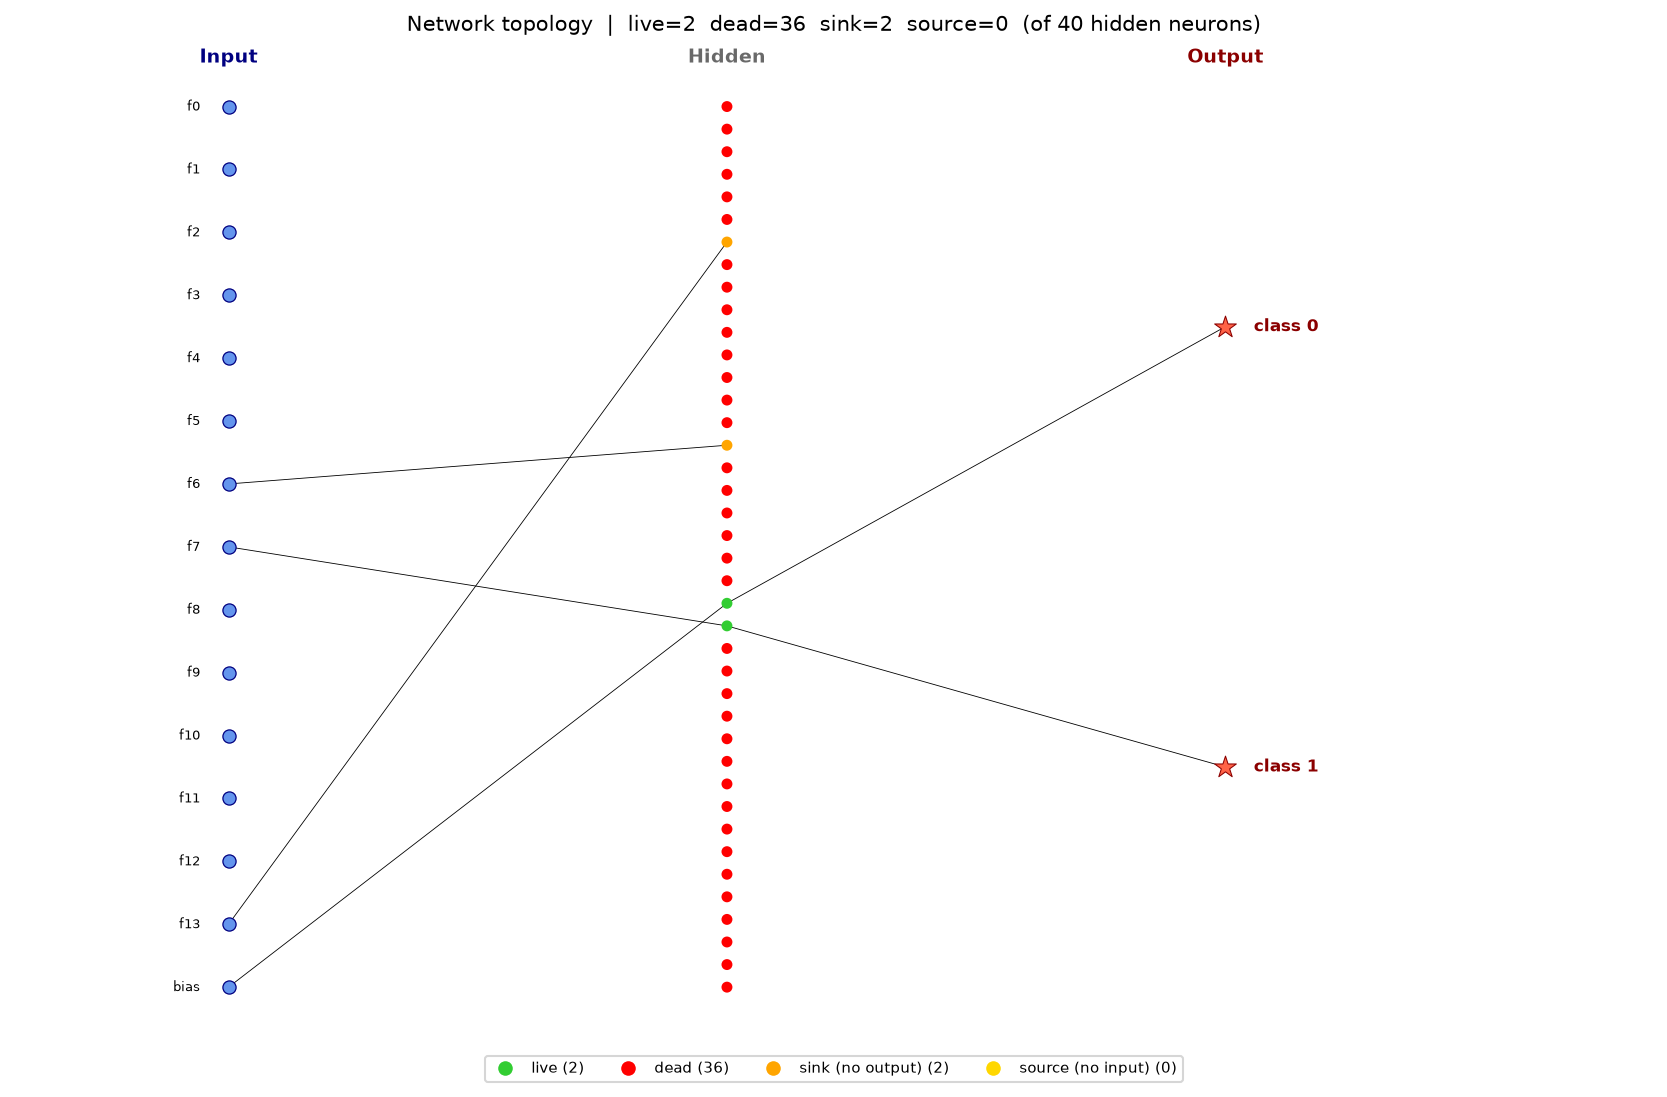
\includegraphics[width=\textwidth]{images/conectividad_ds1_moeackf.png}
    \caption{ds1-MOEA-CKF (corrida 3). Fila 1 de la Tabla~\ref{tab:conectividad-combo}.}
    \label{fig:conectividad-ds1-ckf}
\end{subfigure}
\hfill
\begin{subfigure}[b]{0.31\textwidth}
    \centering
    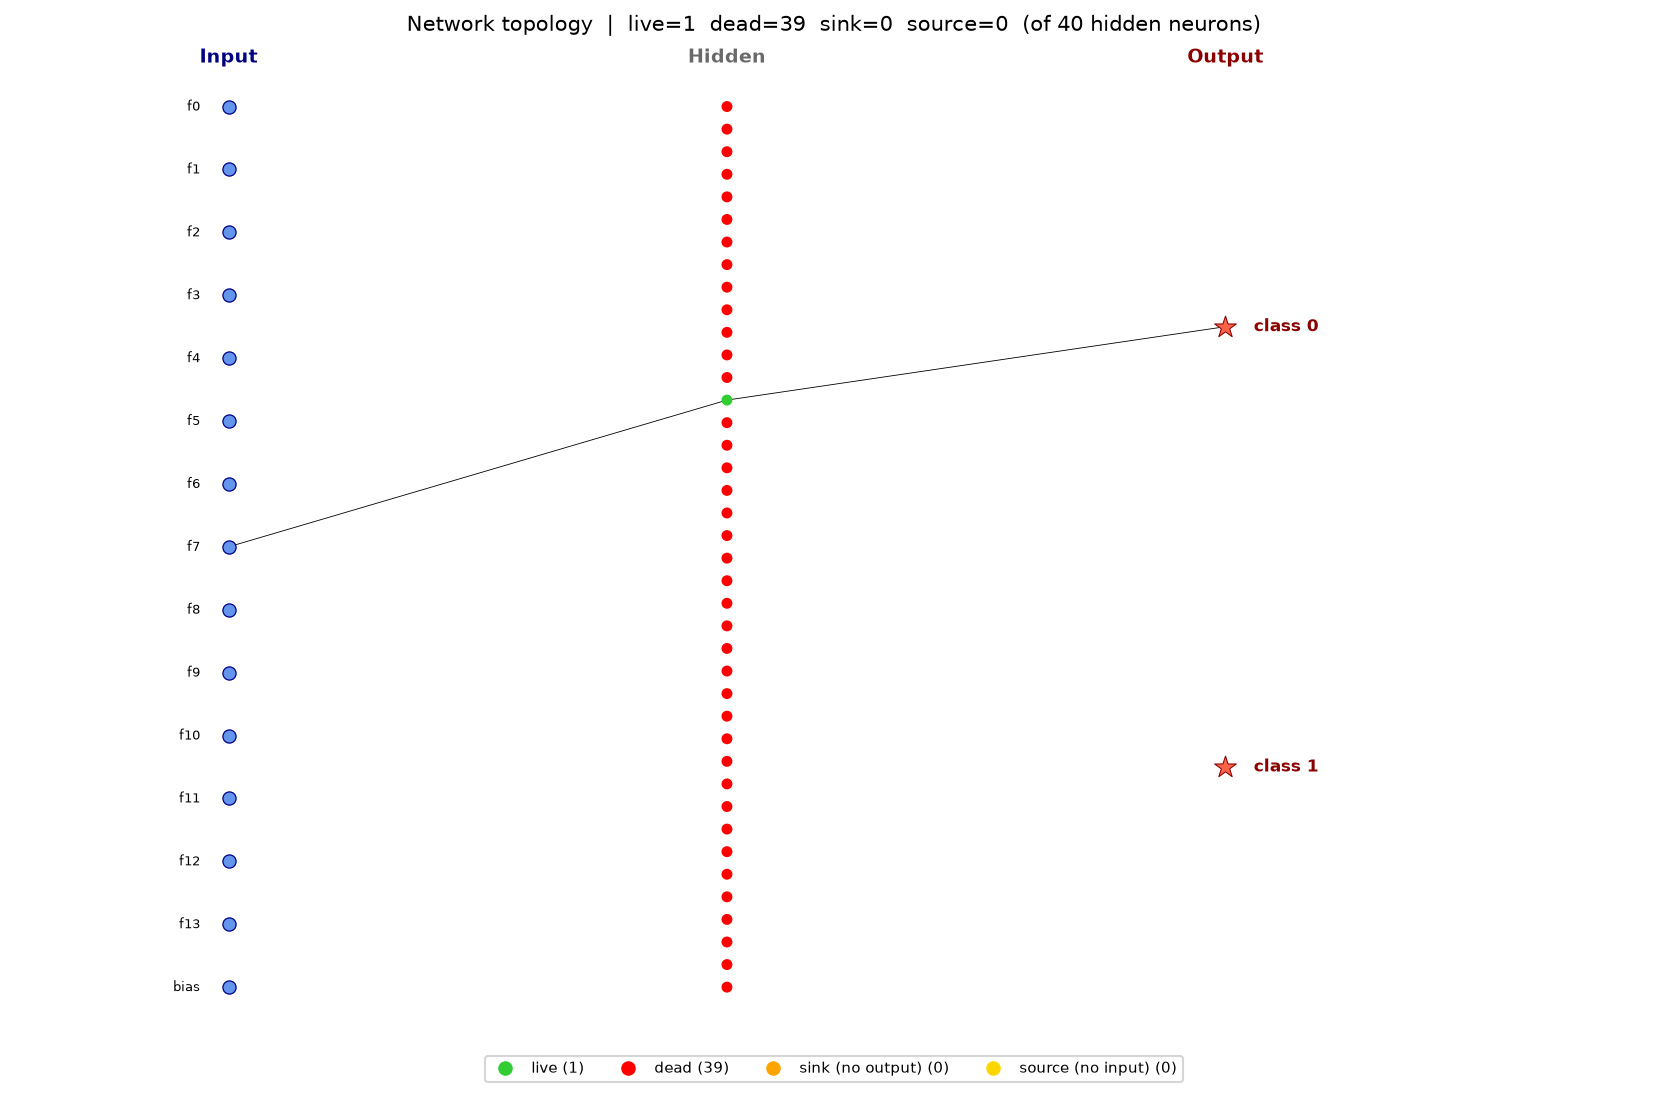
\includegraphics[width=\textwidth]{images/conectividad_ds1_snsgaii.png}
    \caption{ds1-S-NSGA-II (corrida 0). Fila 2 de la Tabla~\ref{tab:conectividad-combo}.}
    \label{fig:conectividad-ds1-nsga}
\end{subfigure}
\hfill
\begin{subfigure}[b]{0.31\textwidth}
    \centering
    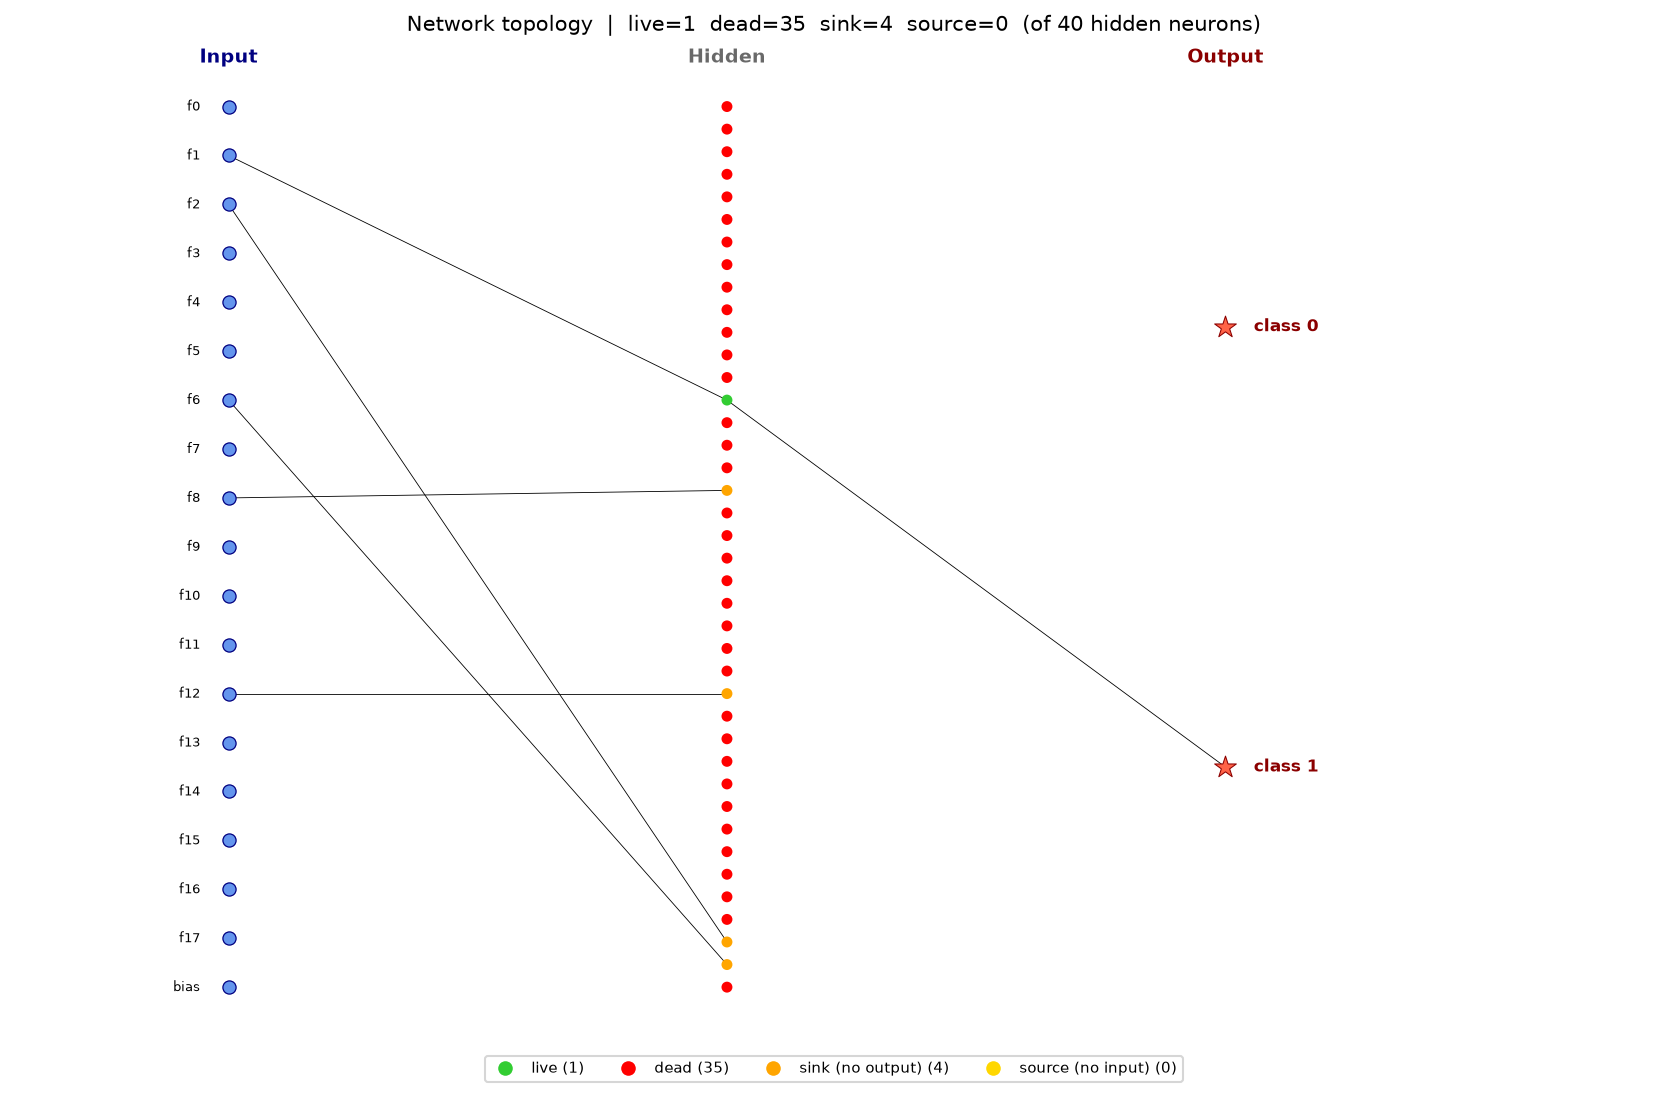
\includegraphics[width=\textwidth]{images/conectividad_ds2_moeackf.png}
    \caption{ds2-MOEA-CKF (corrida 24). Fila 3 de la Tabla~\ref{tab:conectividad-combo}.}
    \label{fig:conectividad-ds2-ckf}
\end{subfigure}

\par\vspace{0.4cm}

% Fila 2
\begin{subfigure}[b]{0.31\textwidth}
    \centering
    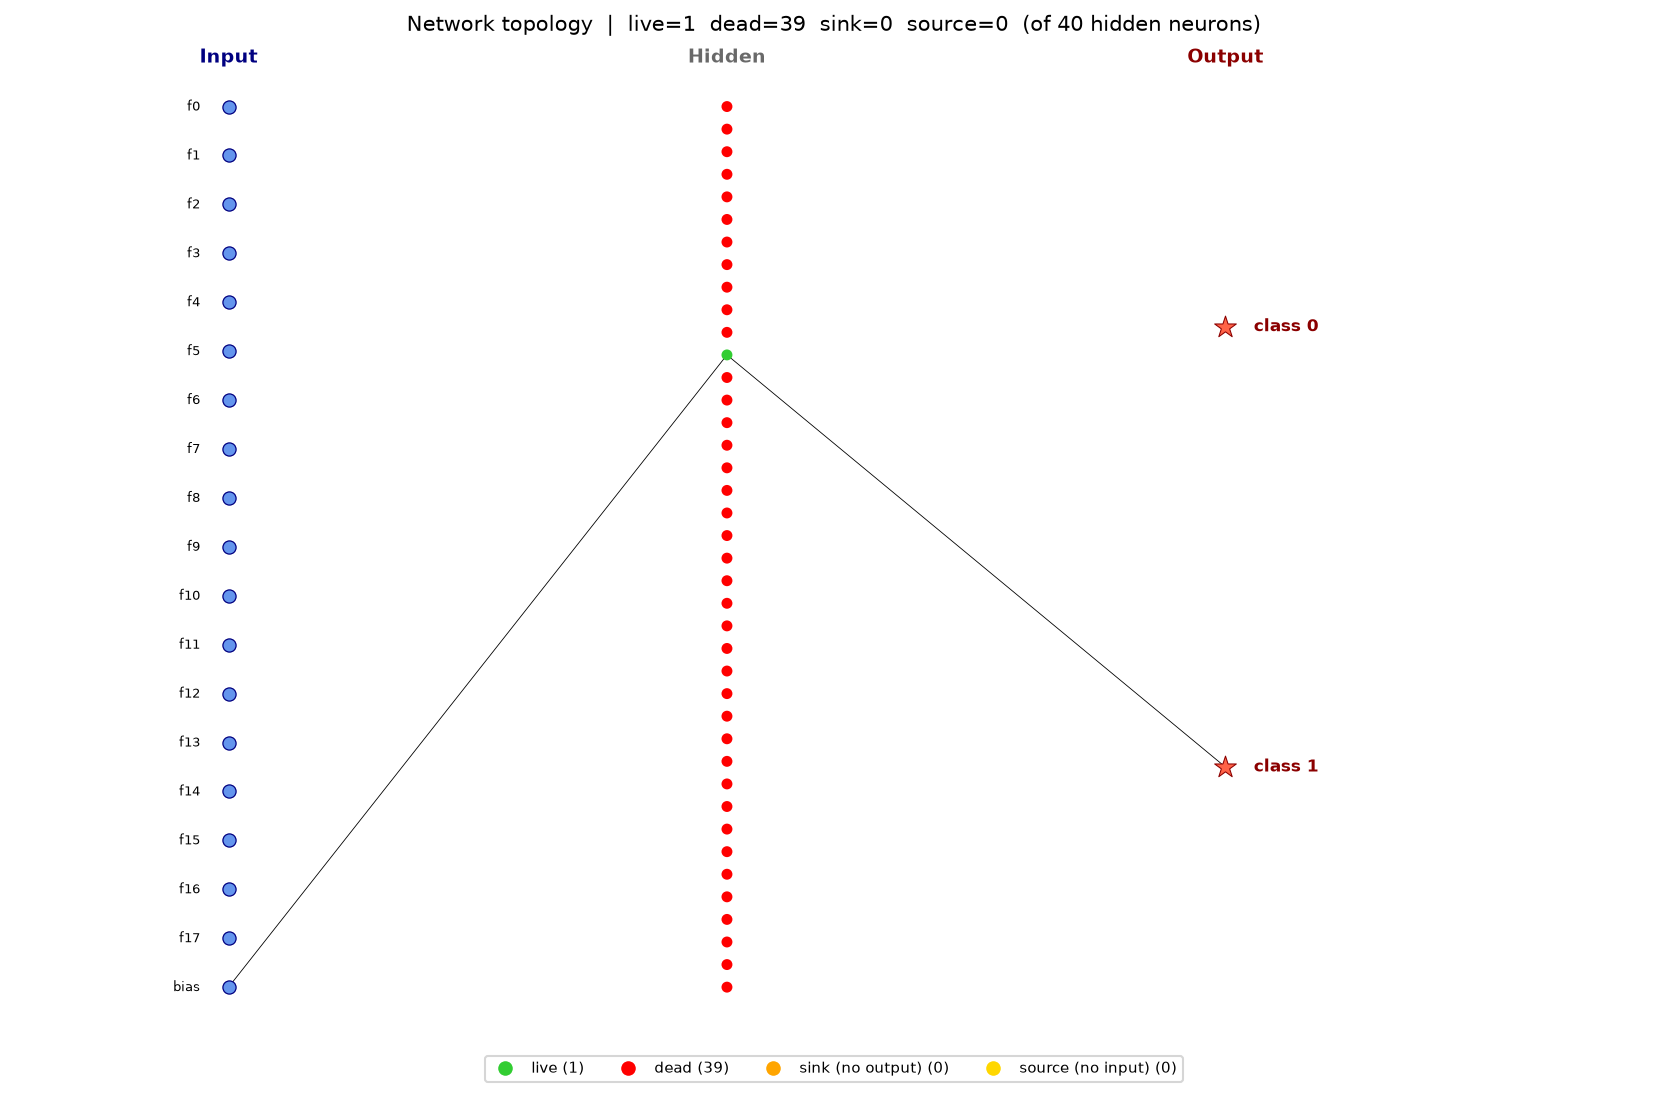
\includegraphics[width=\textwidth]{images/conectividad_ds2_snsgaii.png}
    \caption{ds2-S-NSGA-II (corrida 0). Fila 4 de la Tabla~\ref{tab:conectividad-combo}.}
    \label{fig:conectividad-ds2-nsga}
\end{subfigure}
\hfill
\begin{subfigure}[b]{0.31\textwidth}
    \centering
    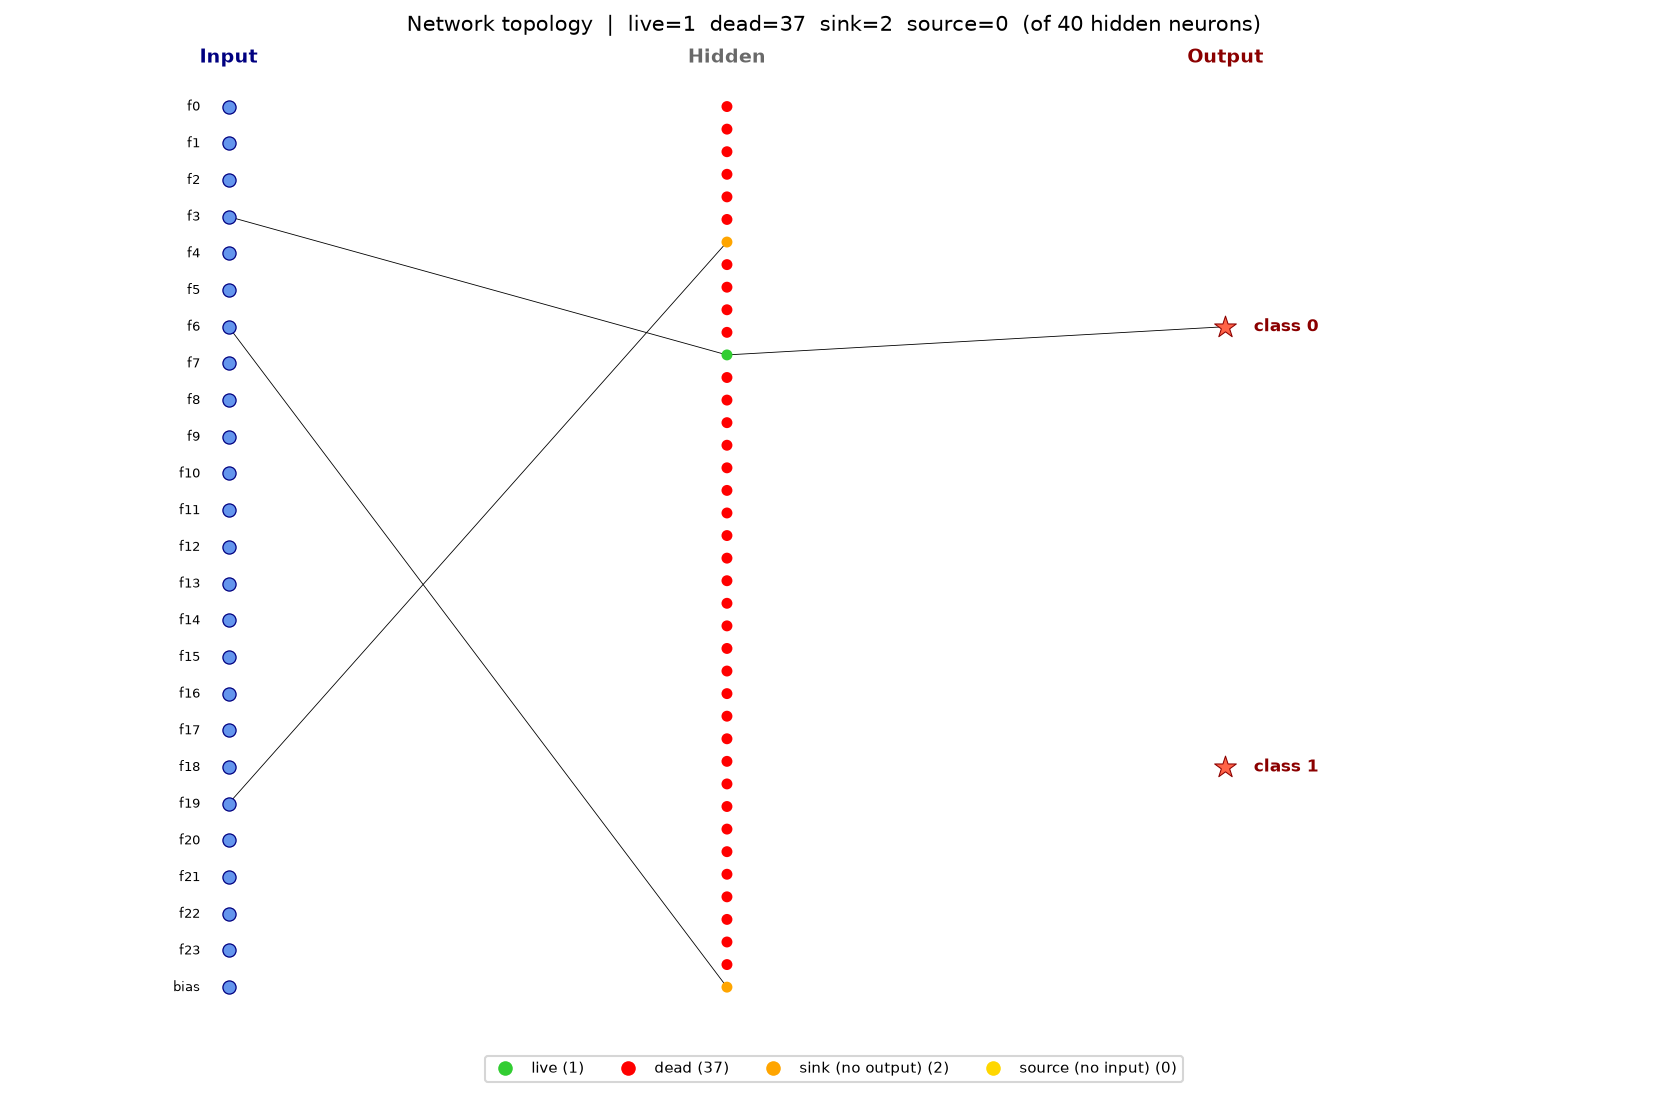
\includegraphics[width=\textwidth]{images/conectividad_ds3_moeackf.png}
    \caption{ds3-MOEA-CKF (corrida 20). Fila 5 de la Tabla~\ref{tab:conectividad-combo}.}
    \label{fig:conectividad-ds3-ckf}
\end{subfigure}
\hfill
\begin{subfigure}[b]{0.31\textwidth}
    \centering
    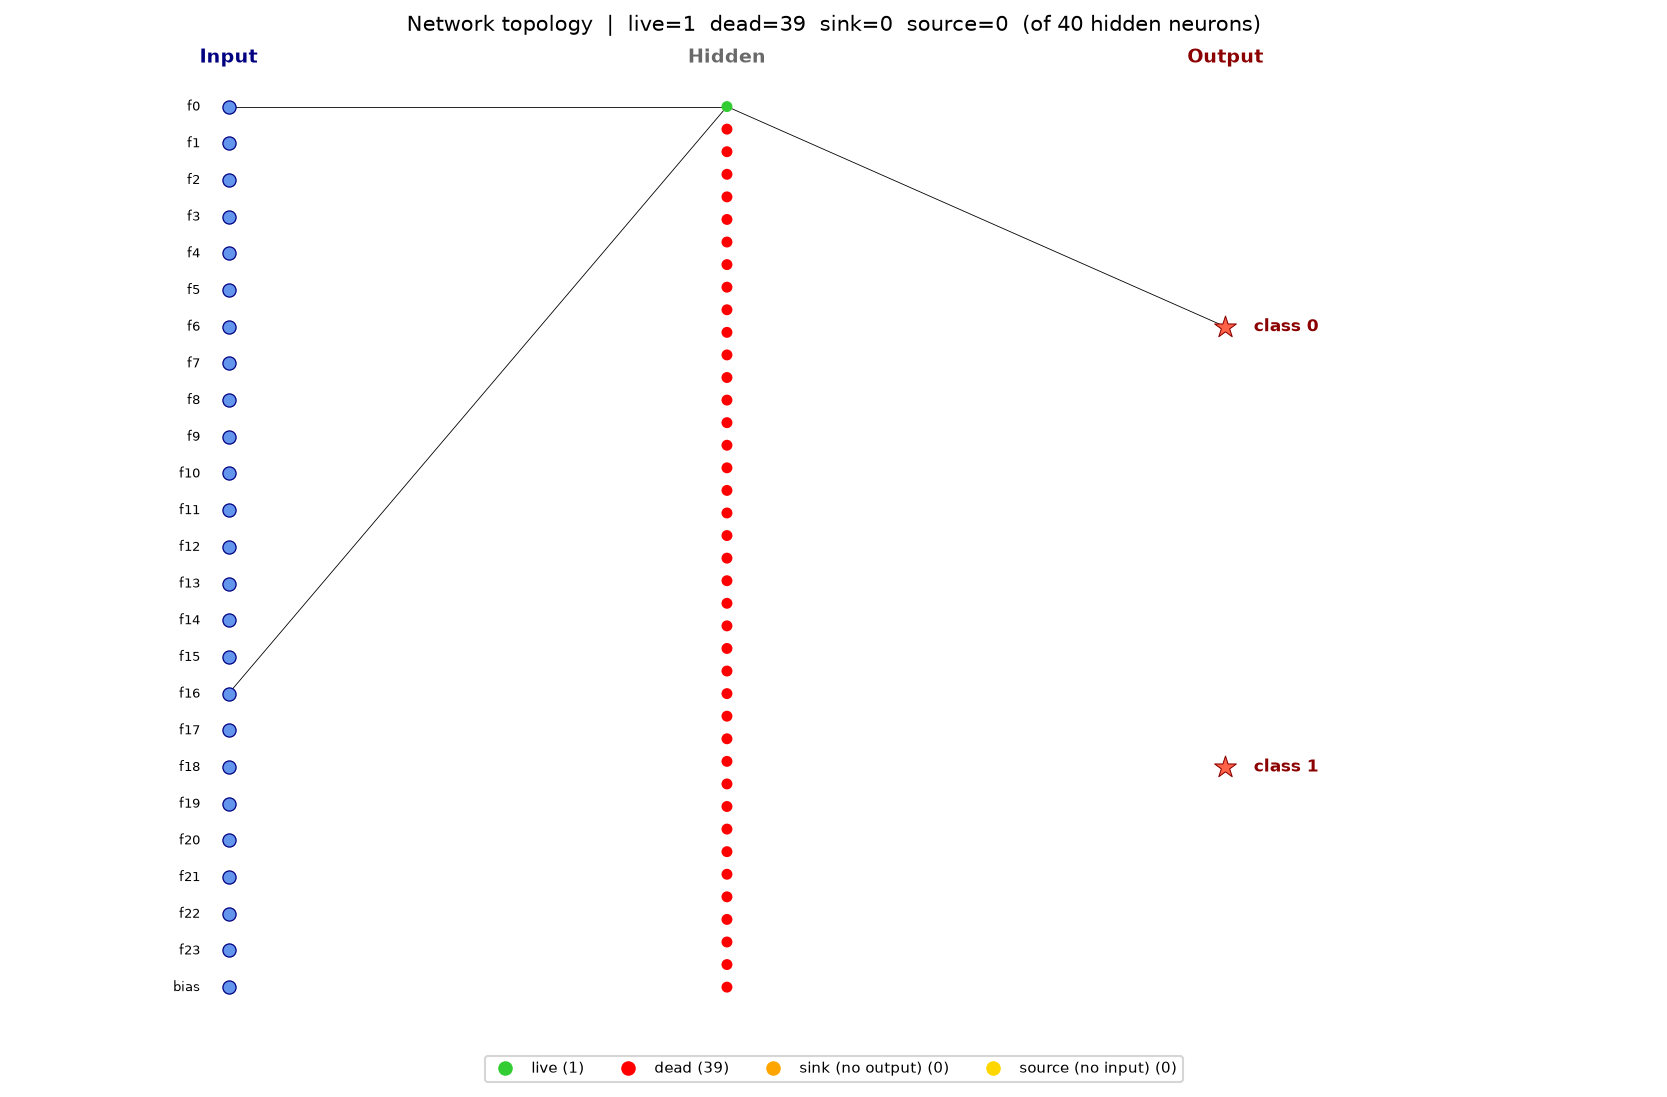
\includegraphics[width=\textwidth]{images/conectividad_ds3_snsgaii.png}
    \caption{ds3-S-NSGA-II (corrida 5). Fila 6 de la Tabla~\ref{tab:conectividad-combo}.}
    \label{fig:conectividad-ds3-nsga}
\end{subfigure}

\caption{Solución de mejor exactitud de una corrida representativa por combinación de dataset y algoritmo, \texttt{ds1}-\texttt{ds3} (\texttt{ds4} en el Anexo~A). Neuronas ocultas: vivas (verde), muertas (roja), sumidero (naranjo) y fuente (amarillo); estrellas rojas: neuronas de salida.}
\label{fig:conectividad-ejemplo}

\end{figure}